\documentclass{beamer}

\usepackage{graphicx}
\usepackage[T1]{fontenc}
\usepackage[utf8]{inputenc}
\usepackage[english]{babel}
\usepackage{lmodern}
\usepackage{ragged2e}
\usepackage{siunitx}
\usepackage{hyperref}
\usepackage{amsmath}
\usetheme[pageofpages=of]{Unipd}

\title{N-Body Simulation: Design, Optimizations and Benchmarking}
\author[Alessio]{Alessio}
\institute{M. Sc. Physics of Data, University of Padova}
\date{July 23, 2025}

\begin{document}

% Title
\frame{\titlepage}

% Index
\begin{frame}{Outline}
    \tableofcontents
\end{frame}

%--- Music ---
%https://open.spotify.com/intl-it/track/7DBHecNdRB8fIQSSRxhqF0?si=77d1995f0f1e40ae


% --- Sections ---
\section{Introduction and Motivation}
\begin{frame}{Introduction and Motivation}
    \begin{itemize}
        \item Started as a simple single-file C++ code for Voyager II trajectory
        \item Evolved into a modular, configurable N-body simulator
        \item Main goals:
        \begin{itemize}
            \item Flexible and extensible framework
            \item Fair CPU vs GPU performance comparison
            \item Advanced optimizations and interactive visualization
        \end{itemize}
    \end{itemize}
\end{frame}

\section{Project Evolution}
\begin{frame}{Project Evolution}
    \begin{itemize}
        \item Initial single-file C++ implementation
        \item Output separation and modularization
        \item Integration of OpenMP, CUDA, (AVX2)
        \item Refactoring, CMake build system, JSON configuration
        \item Interactive visualization with OpenGL
    \end{itemize}
\end{frame}

%\section{General Architecture}
%\begin{frame}{General Architecture}
%    \begin{itemize}
%        \item \textbf{Core}: simulation logic, data structures, and CPU part
%        \item \textbf{CUDA}: GPU kernels, utilities and host functions
%        \item \textbf{Visualization}: OpenGL and OpenGL/CUDA interop
%        \item \textbf{Output}: CSV output, dynamical buffer to use for other integrations
%        \item \textbf{Configuration}: single JSON file
%    \end{itemize}
%    \vspace{1em}
%
%\end{frame}

%\begin{frame}
%    \begin{center}
%        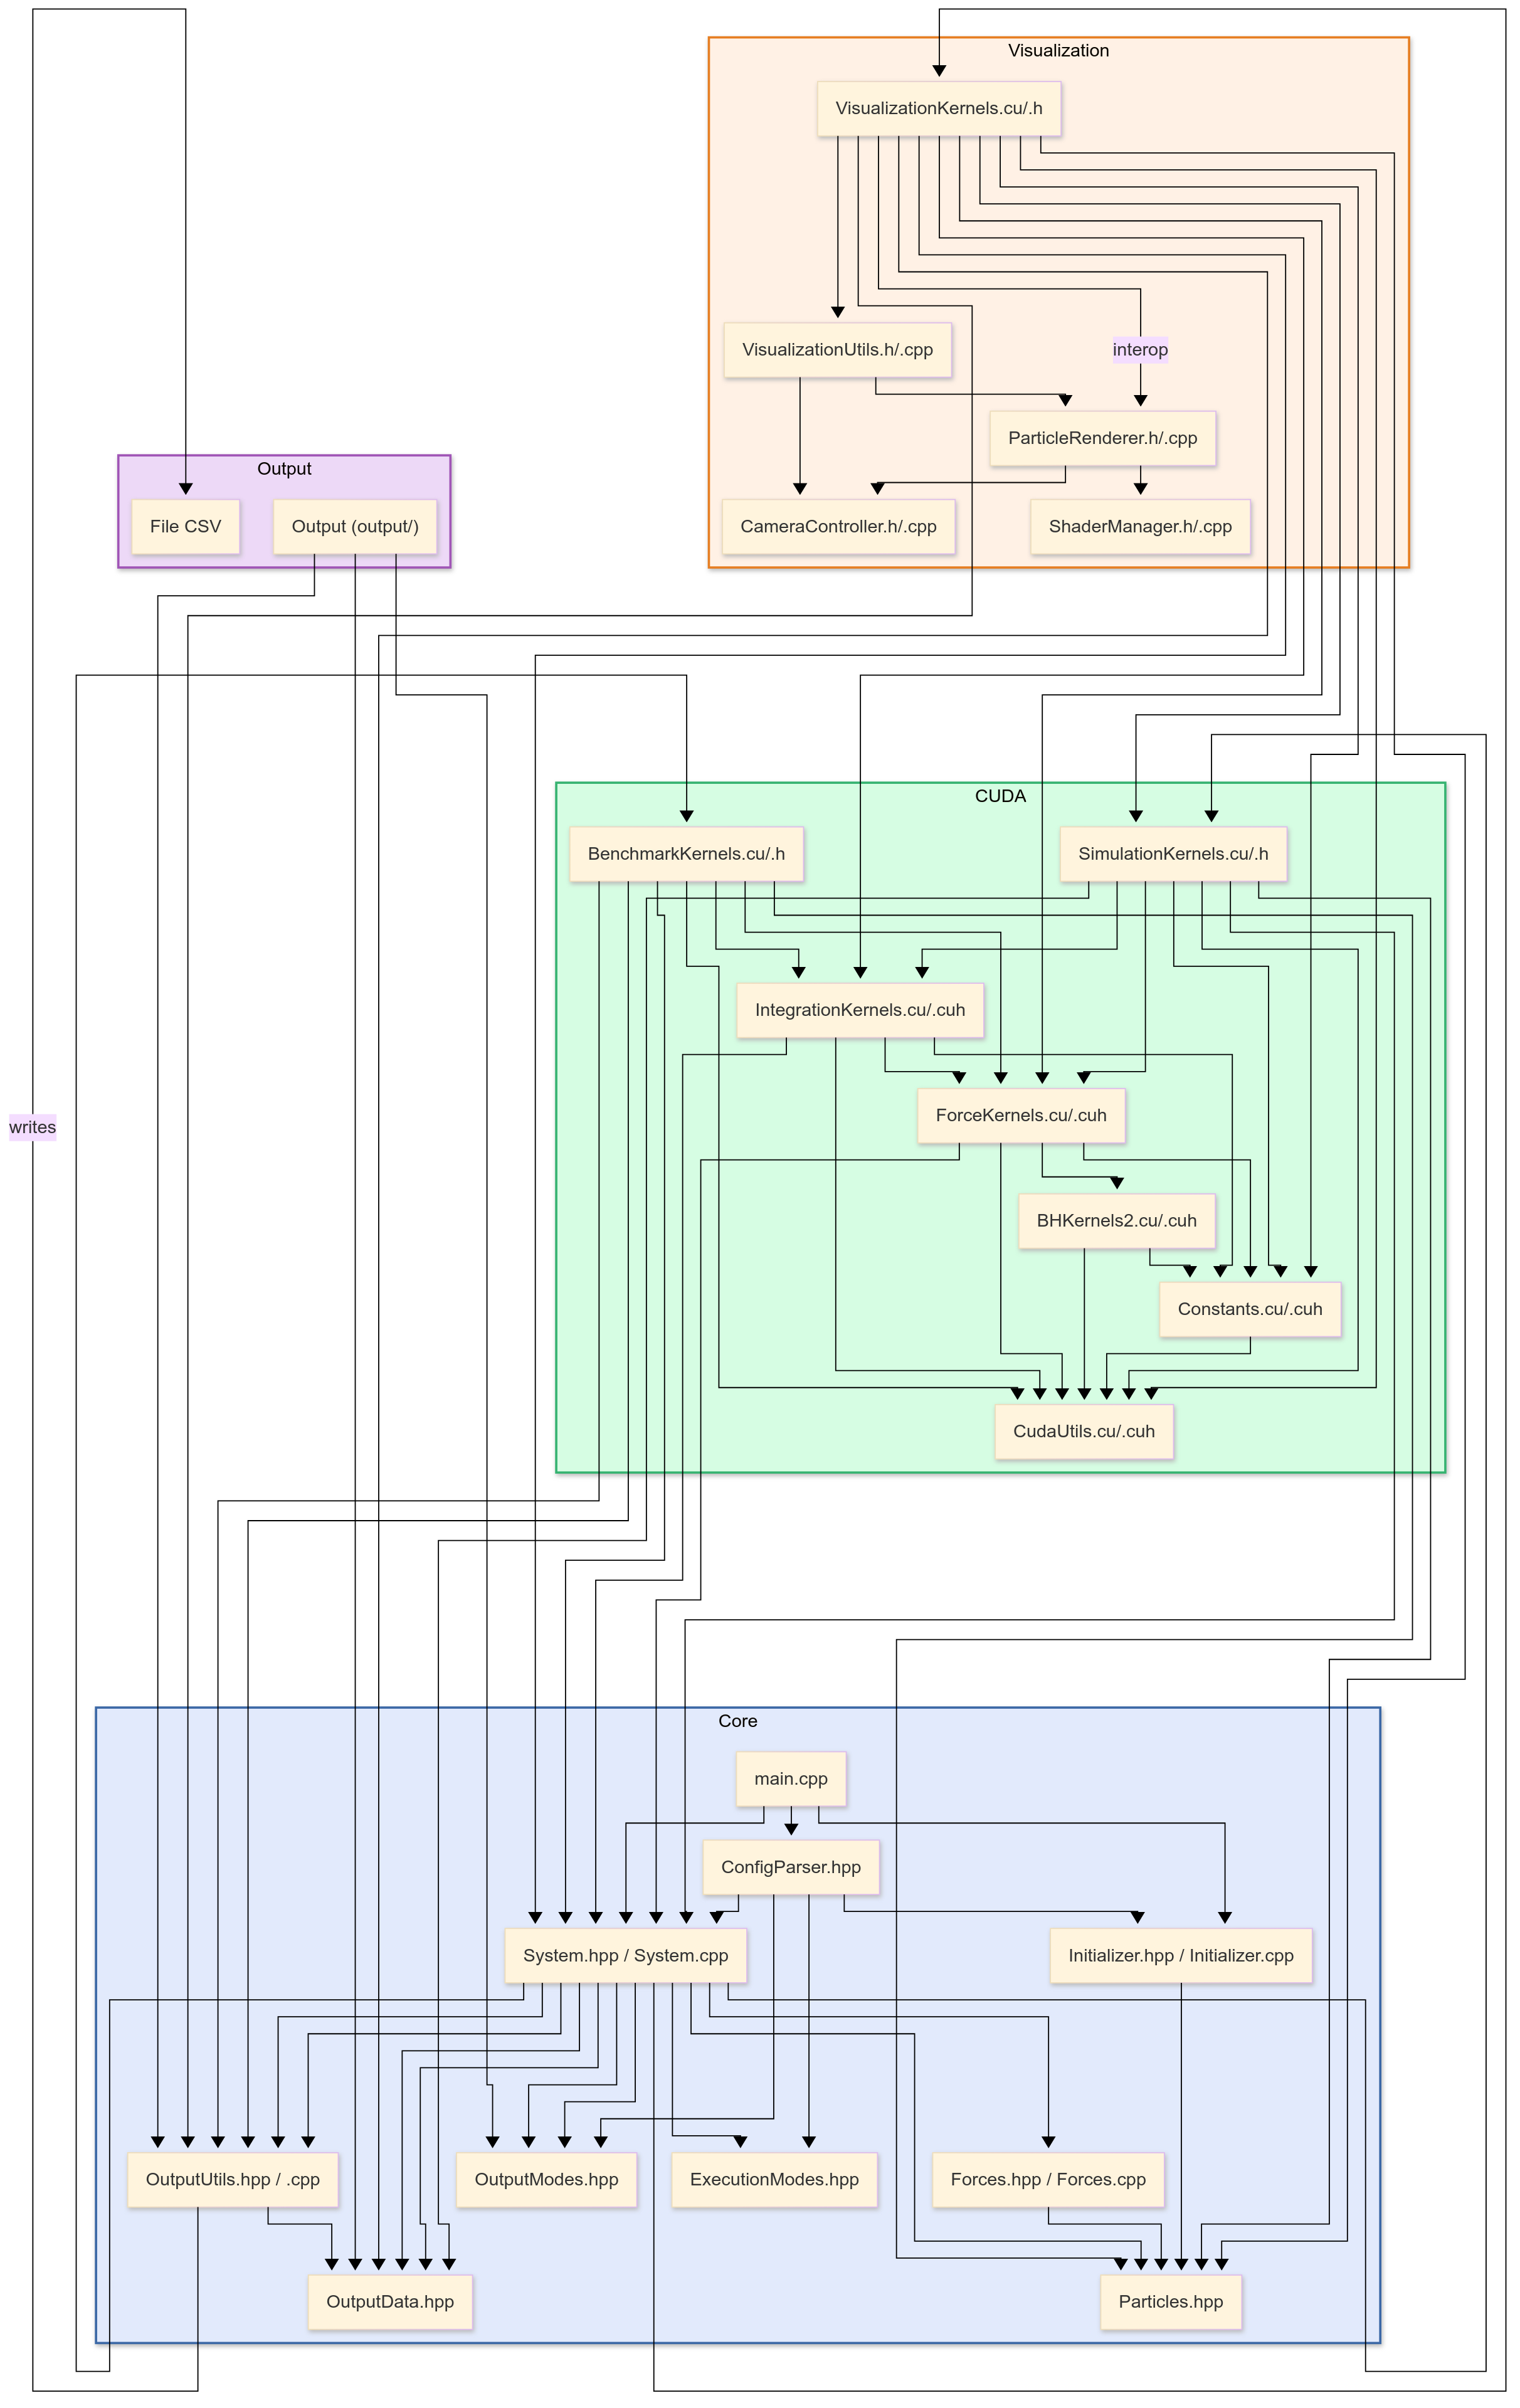
\includegraphics[width=0.5\textwidth]{figures/mermaid_chart.png}
%    \end{center}
%\end{frame}

\begin{frame}{General Architecture}
    \begin{columns}[c]
        \column{0.4\textwidth}
            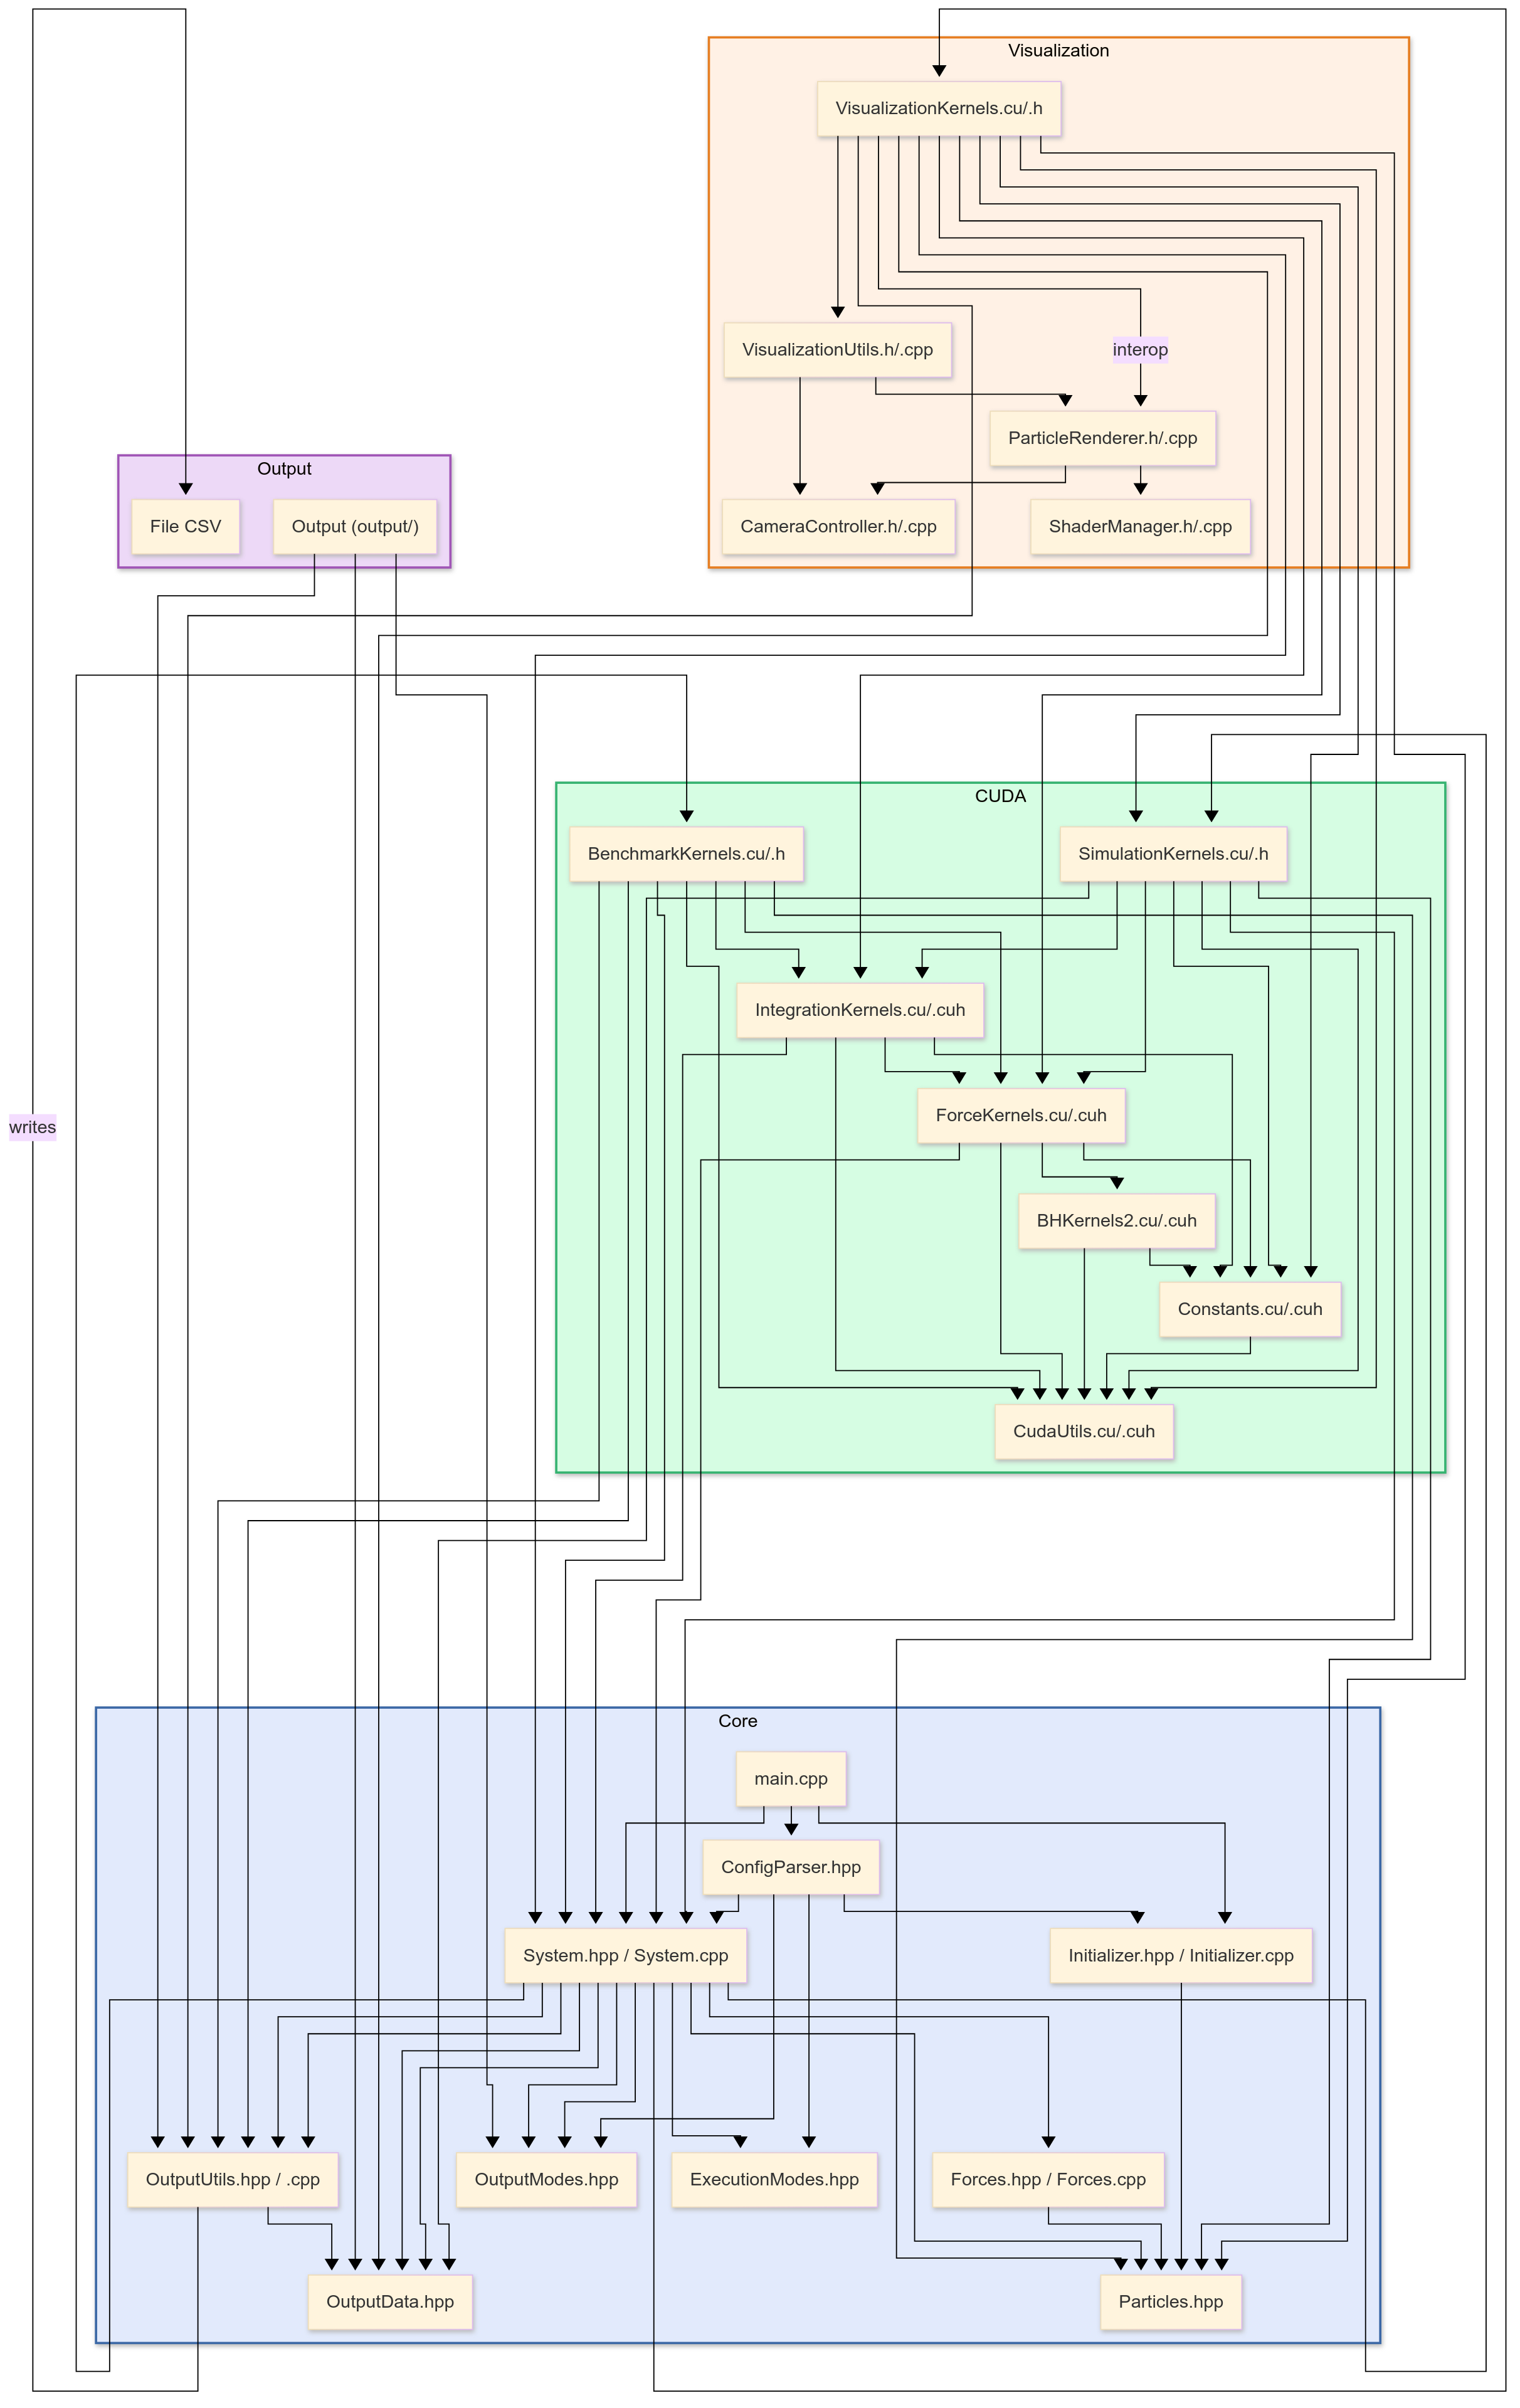
\includegraphics[width=\linewidth]{figures/mermaid_chart.png}
        \column{0.6\textwidth}
            \begin{itemize}
                \item \textbf{Core}: simulation logic, data structures, and CPU part
                \item \textbf{CUDA}: GPU kernels, utilities and host functions
                \item \textbf{Visualization}: OpenGL and OpenGL/CUDA interop
                \item \textbf{Output}: CSV output, dynamical buffer to use for other integrations
                \item \textbf{Configuration}: single JSON file
            \end{itemize}
    \end{columns}
\end{frame}

\begin{frame}{Configuration and Initialization}
    \begin{itemize}
        \item Single JSON configuration file
        \item Flexible initialization: random, file-based, or custom implementations (galaxy, stellar systems, etc.)
    \end{itemize}
    \vspace{1em}
    \begin{columns}[c]
        \column{0.48\textwidth}
            \centering
            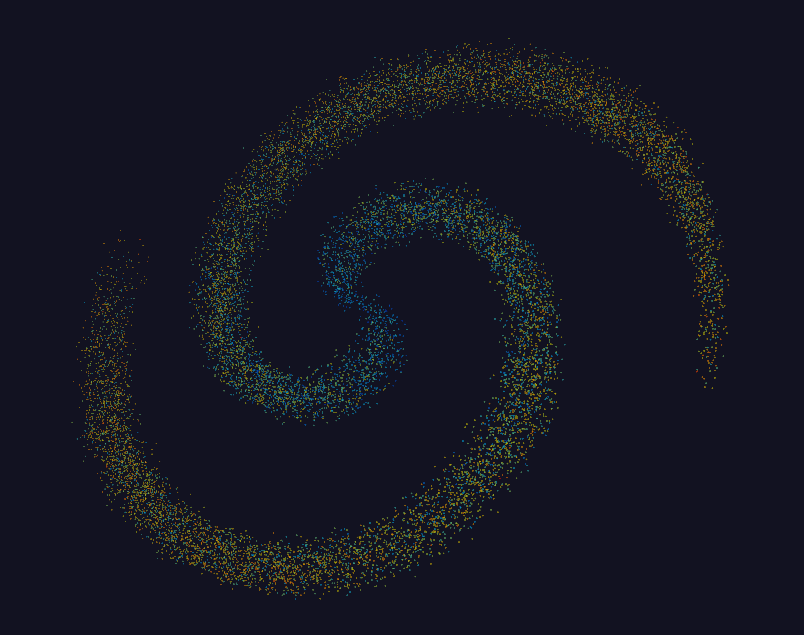
\includegraphics[width=\linewidth]{figures/galaxy_2.png}\\
            \small Example of a galaxy configuration
        \column{0.04\textwidth}
            % Spazio tra le immagini
        \column{0.48\textwidth}
            \centering
            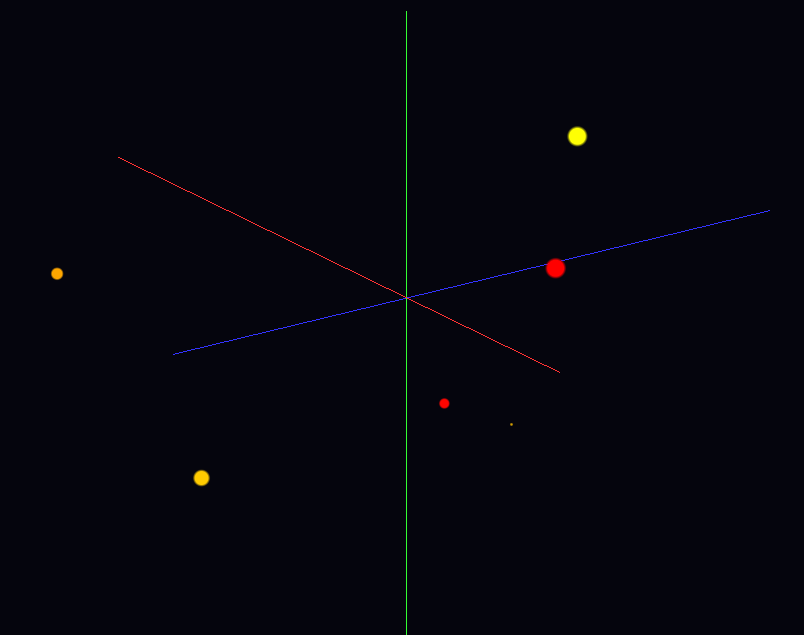
\includegraphics[width=\linewidth]{figures/random.png}\\
            \small Example of random initialization
    \end{columns}
\end{frame}

\section{Memory Management and Optimizations}
\begin{frame}{Memory Management and Optimizations}
    \begin{itemize}
        \item Structure of Arrays (SoA) for efficient access and fully coalesced memory with double4
        \item Pinned memory and CUDA streams
        \item AVX2 vectorization and OpenMP threading
        \item Low-ish memory footprint: \SI{1.1}{GiB} for 1B particles
        \item In CSV output mode, System is copied only at the start $\rightarrow$ multiple cuda streams for memory and compute management.
        \item In visualization mode, System is copied every frame to a dynamic buffer, which is then used for rendering
                $\rightarrow$ worst case scenario $\Rightarrow$ OpenGL-cuda interop and separate rendering stream $\rightarrow$ less bottleneck.
    \end{itemize}
\end{frame}

\section{Force and Integration Methods}
\begin{frame}{Force and Integration Methods}
    \begin{itemize}
        \item Pairwise, Adaptive Mutual Softening, Barnes-Hut (no GPU implementation)
        \item Configurable physical constants and softening
        \item Multiple integration schemes: Euler (not symplectic), Velocity Verlet (symplectic)
    \end{itemize}
    \vspace{1em}
    \begin{center}
    \scriptsize
    \begin{tabular}{cc}
        \textbf{Pairwise Newtonian:} &
        \textbf{Adaptive Mutual Softening:} \\
        $\displaystyle
        \vec{a}_i = G \sum_{j \neq i} m_j \frac{\vec{r}_j - \vec{r}_i}{|\vec{r}_j - \vec{r}_i|^3}
        $ 
        &
        $\displaystyle
        \vec{a}_i = G \sum_{j \neq i} m_j \frac{\vec{r}_j - \vec{r}_i}{\left(|\vec{r}_j - \vec{r}_i|^2 + \epsilon_{ij}^2\right)^{3/2}}
        $
        \\[1.5em]
        &
        $\displaystyle
        \epsilon_{ij} = \max\left(\eta\, |\vec{r}_j - \vec{r}_i| \left(\frac{m_i + m_j}{3 \langle m \rangle}\right)^{1/3},\, \epsilon_{\text{min}}\right)
        $
    \end{tabular}
    \end{center}
    \vspace{0.5em}
    {\footnotesize
    where $G$ is the gravitational constant, $\epsilon_{ij}$ is the adaptive softening, $\eta$ and $\epsilon_{\text{min}}$ are tunable parameters, and $\langle m \rangle$ is the average mass.
    }
\end{frame}

\begin{frame}{Block Size Auto-Tuning}
    % Top: Text description
    \begin{itemize}
        \item \textbf{block size selection} is crucial for GPU efficiency in these problems.
        \item Two strategies compared:
        \begin{itemize}
            \item \textcolor{blue}{Occupancy API} (NVIDIA)
            \item \textcolor{red}{Heuristic} (custom, optimized for this workload)
        \end{itemize}
    \end{itemize}
    \vspace{0.5em}
    % Bottom: Two graphs side by side
    \begin{columns}[c]
        \column{0.5\textwidth}
            \centering
            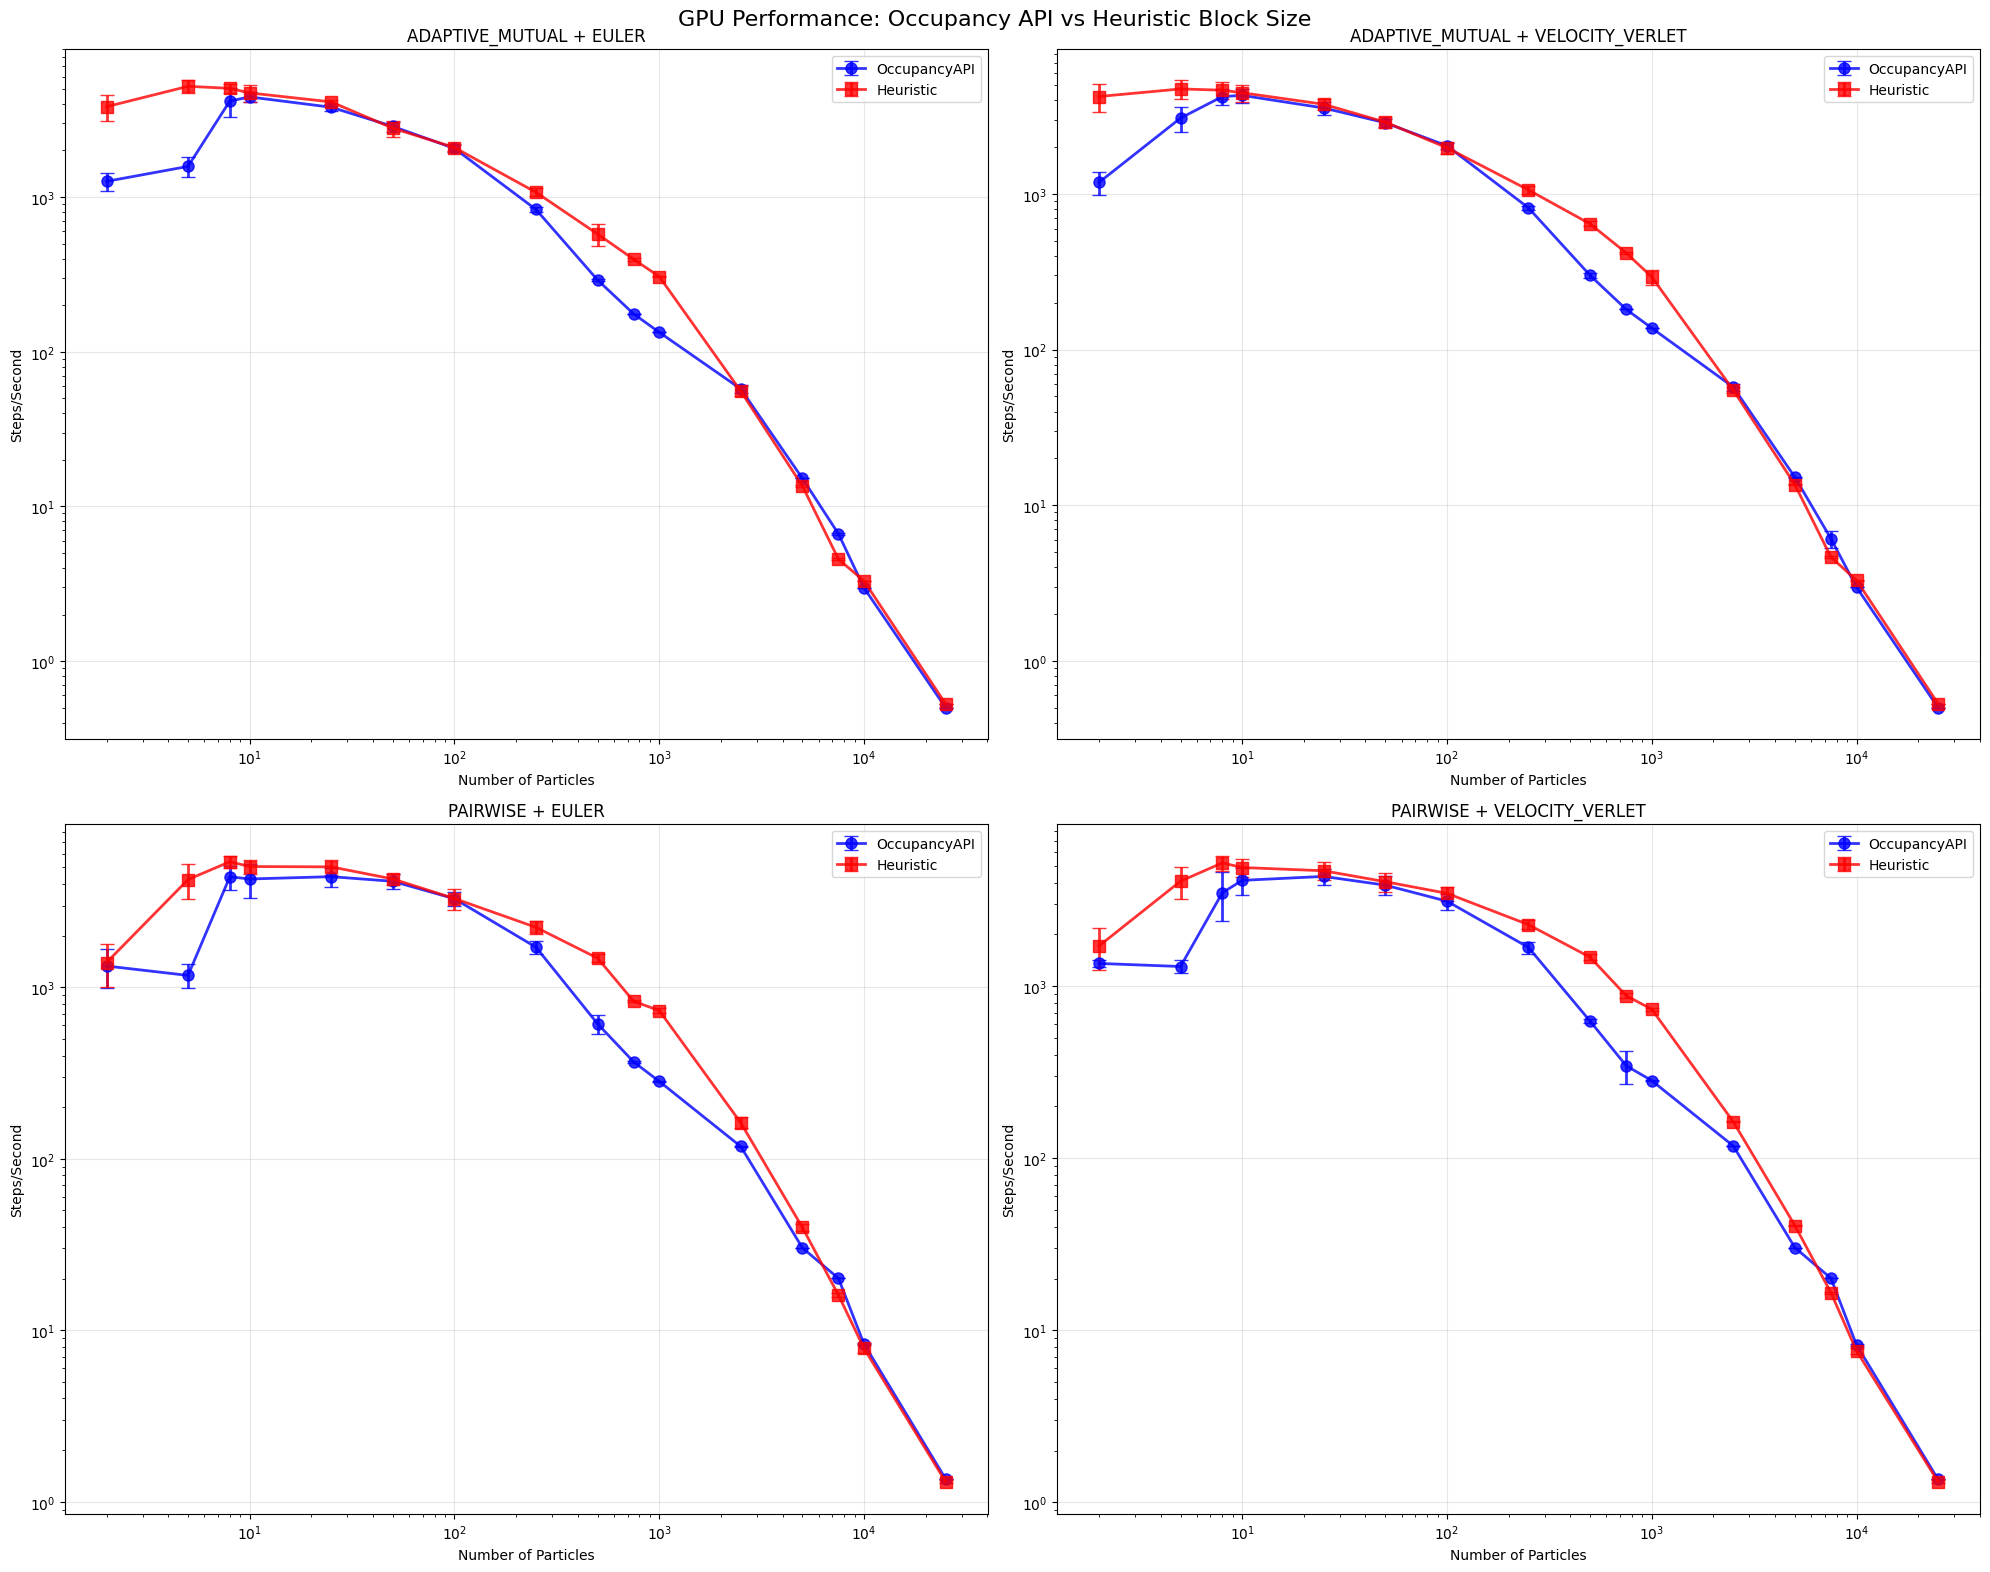
\includegraphics[width=0.99\linewidth]{figures/gpu_perf_blocksize.png}
            %\\[-0.5em]
            %{\scriptsize Performance}
        \column{0.5\textwidth}
            \centering
            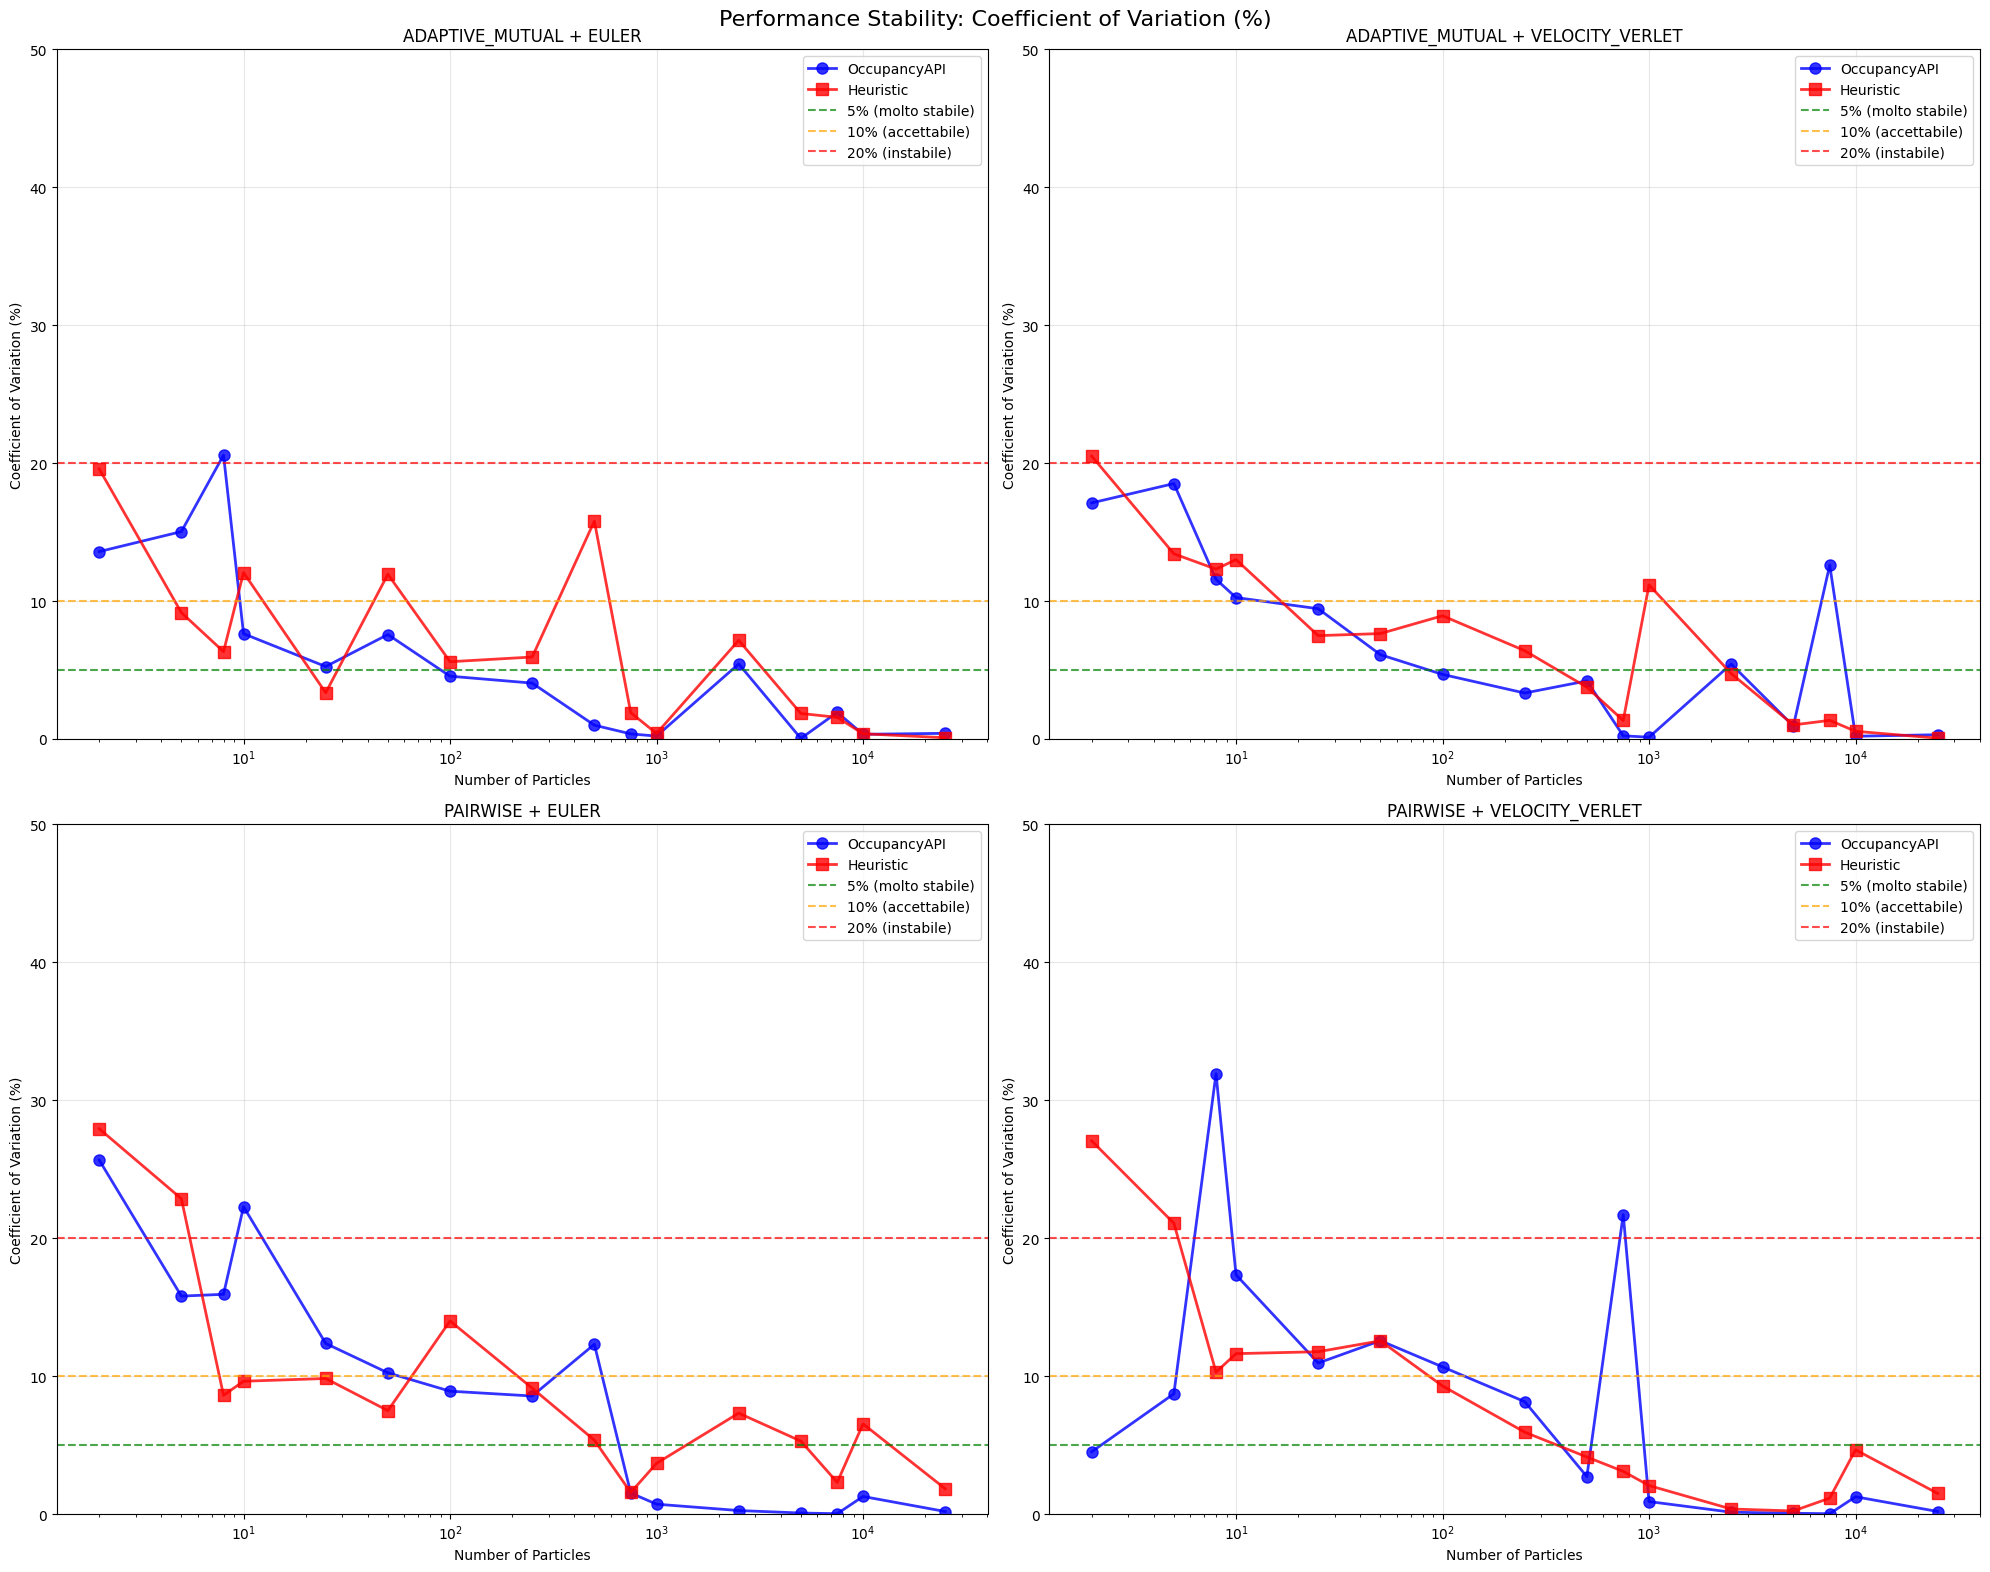
\includegraphics[width=0.99\linewidth]{figures/gpu_stability_blocksize.png}
            %\\[-0.5em]
            %{\scriptsize Stability (CV)}
    \end{columns}
\end{frame}

\begin{frame}{Block Size Auto-Tuning}
    \begin{columns}[c]
        \column{0.6\textwidth}
            {\footnotesize
            Grid size:
            \[
                \text{gridSize} = \left\lceil \frac{n}{\text{blockSize}} \right\rceil
            \]  
            The heuristic is robust, saturates SMs, and respects shared memory limits.  
            The grid size formula is exact for 1D N-body kernels.
            }
            \vspace{0.5cm}
            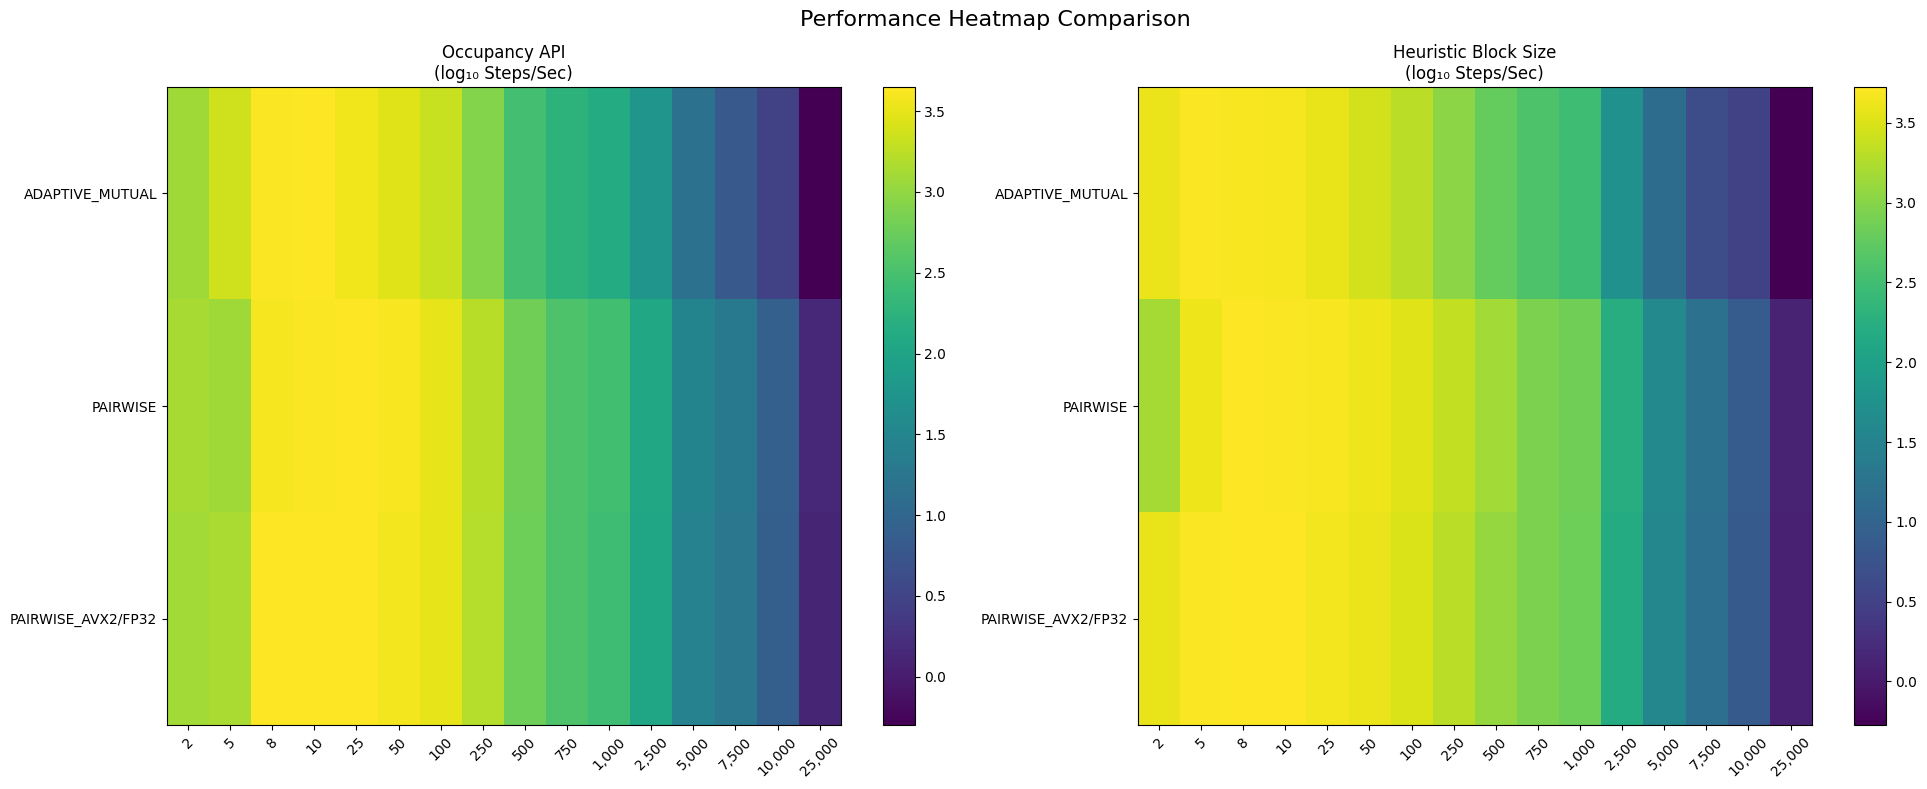
\includegraphics[width=\linewidth]{figures/gpu_heatmap_blocksize.png}
        \column{0.4\textwidth}
            \scriptsize
            \small\begin{block}{Heuristic Block Size Selection (pseudocode)}
            {\ttfamily\footnotesize
            blockSize = 1024 \\
            if n $\leq$ 32: return 32 \\
            while sharedMem(blockSize) $>$ maxShared \&\& blockSize $>$ warp: \\
            \hspace{1em} blockSize //= 2 \\
            blockSize = min(blockSize, maxThreads) \\
            while numBlocks(blockSize) $<$ 2*numSMs \&\& blockSize $>$ warp: \\
            \hspace{1em} blockSize //= 2 \\
            blockSize = max(blockSize, warp) \\
            return blockSize
            }
            \end{block}
    \end{columns}
\end{frame}

\begin{frame}{Basic CPU-GPU Comparison Benchmark}
    \centering
    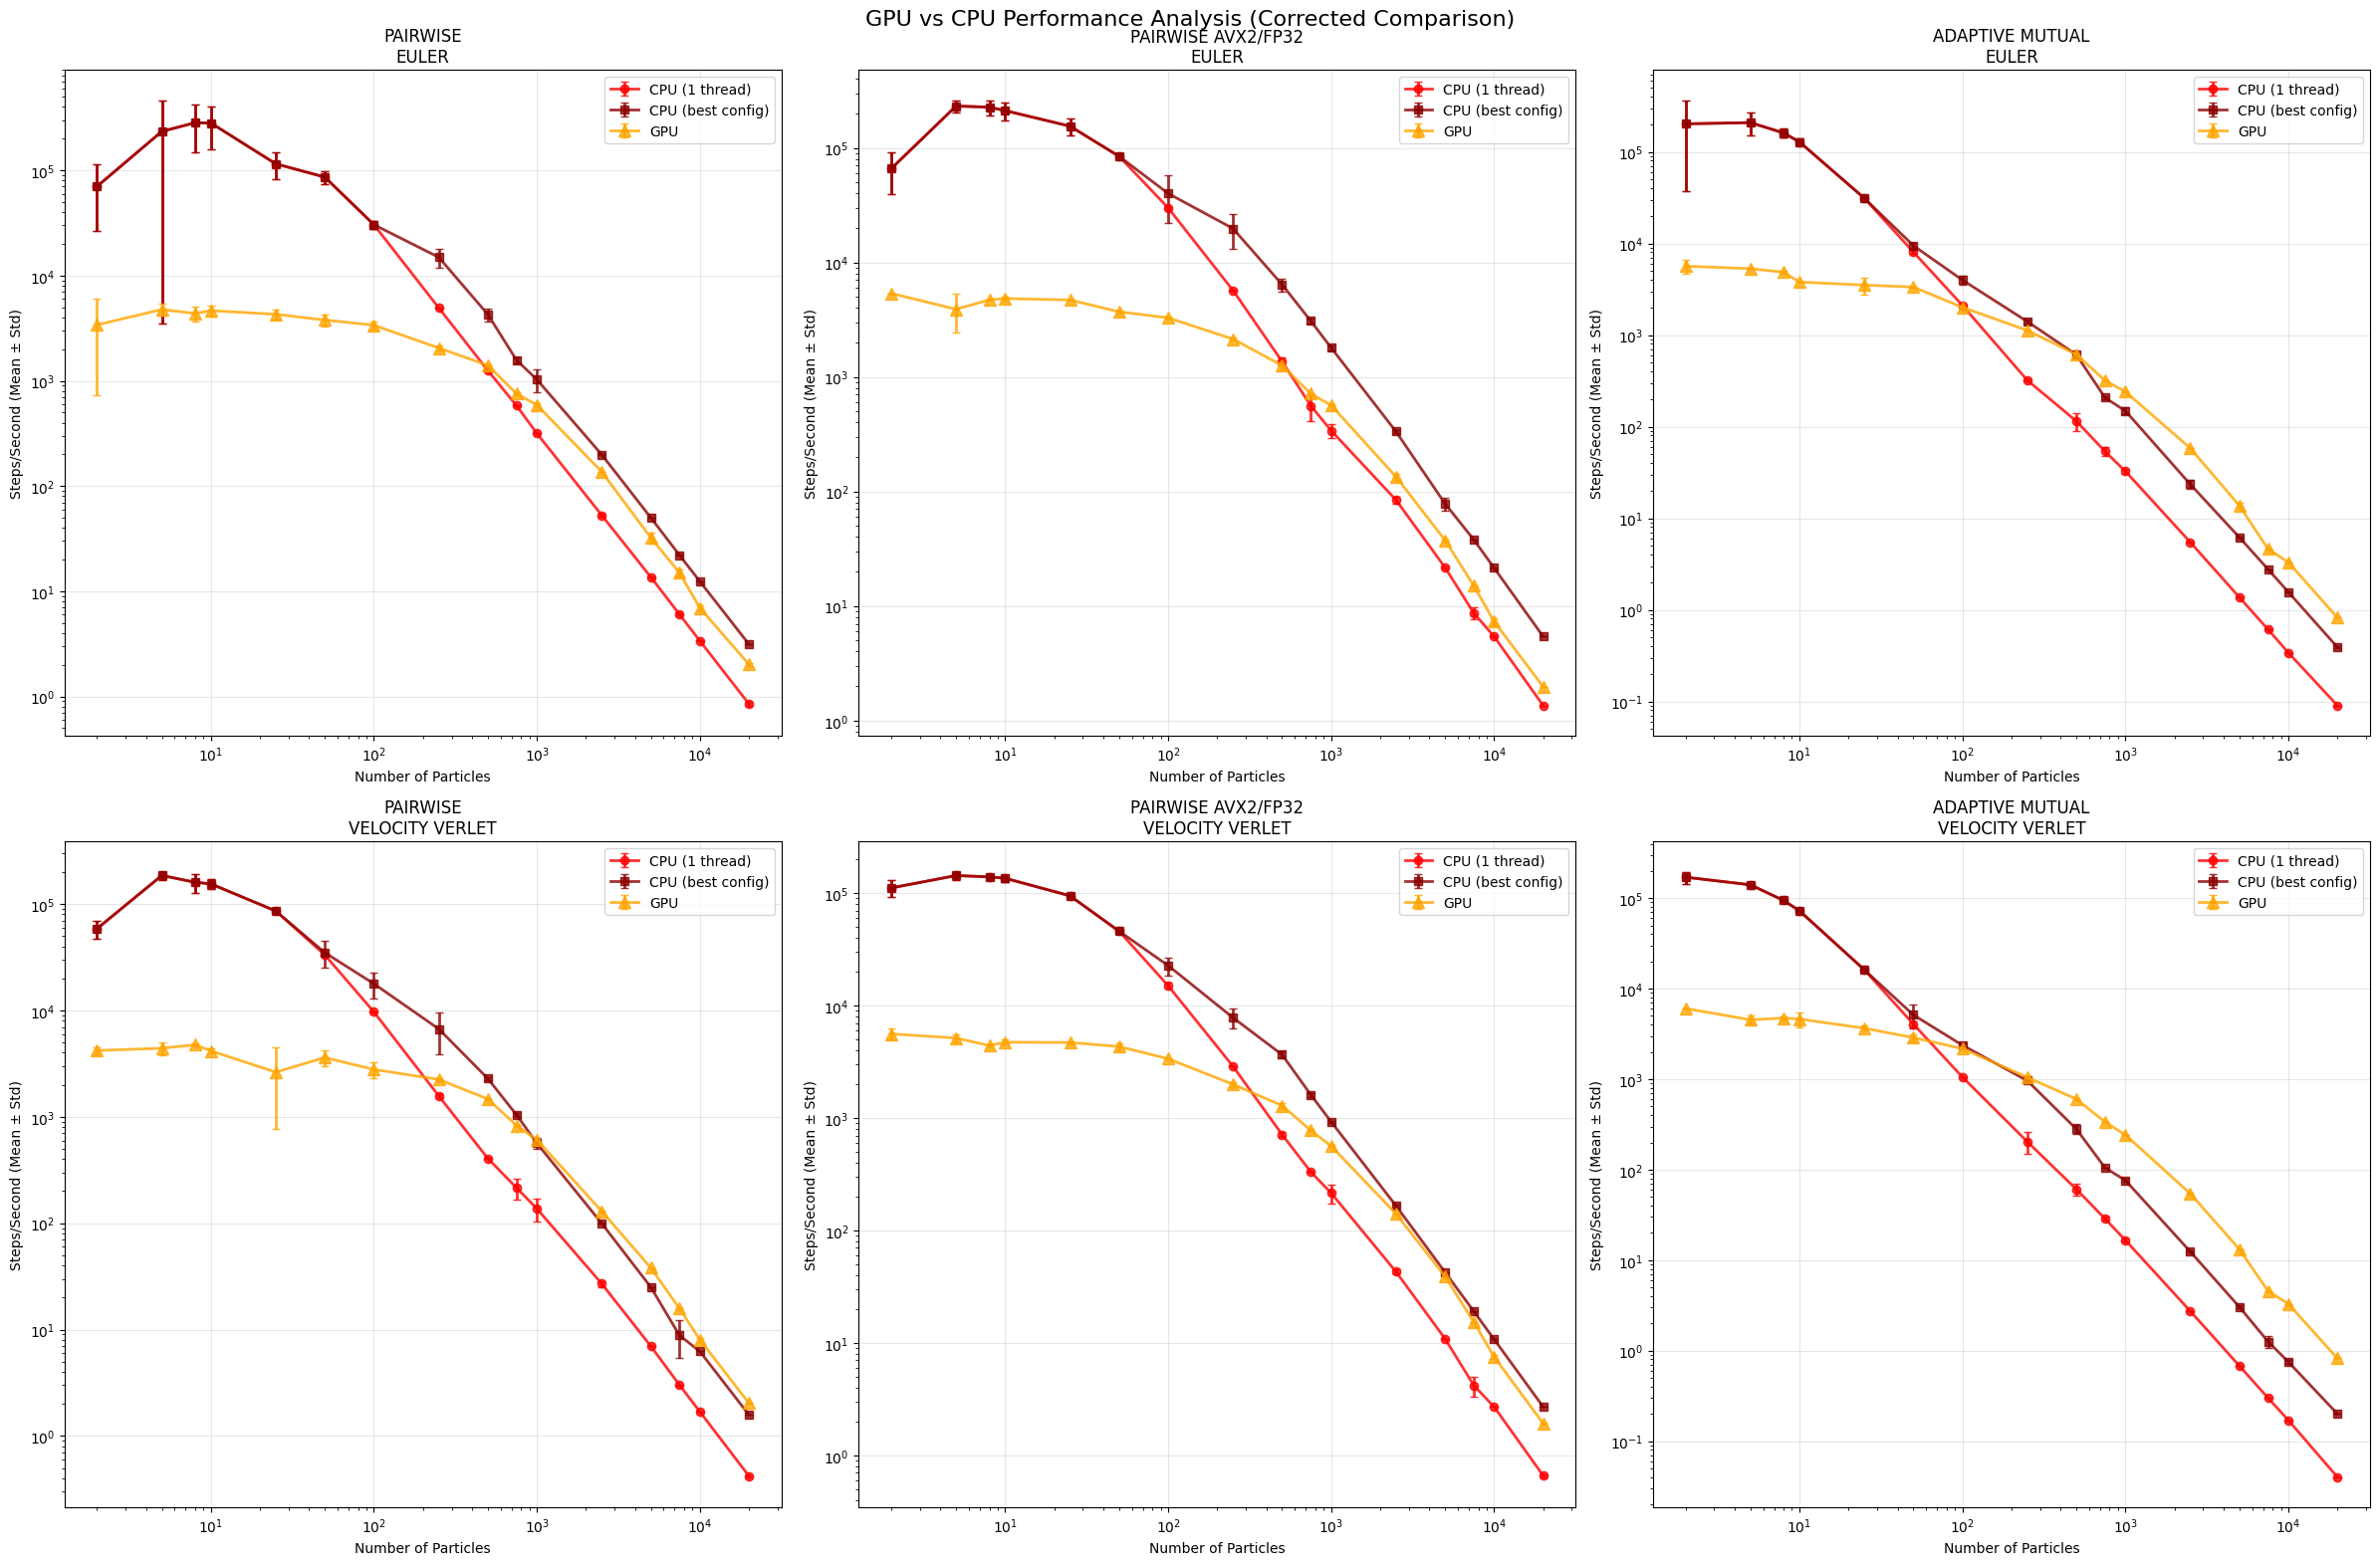
\includegraphics[width=0.99\linewidth]{figures/basic_GPU_CPU_perf.png}
\end{frame}

\begin{frame}{Basic CPU-GPU Comparison Benchmark}
    \centering
    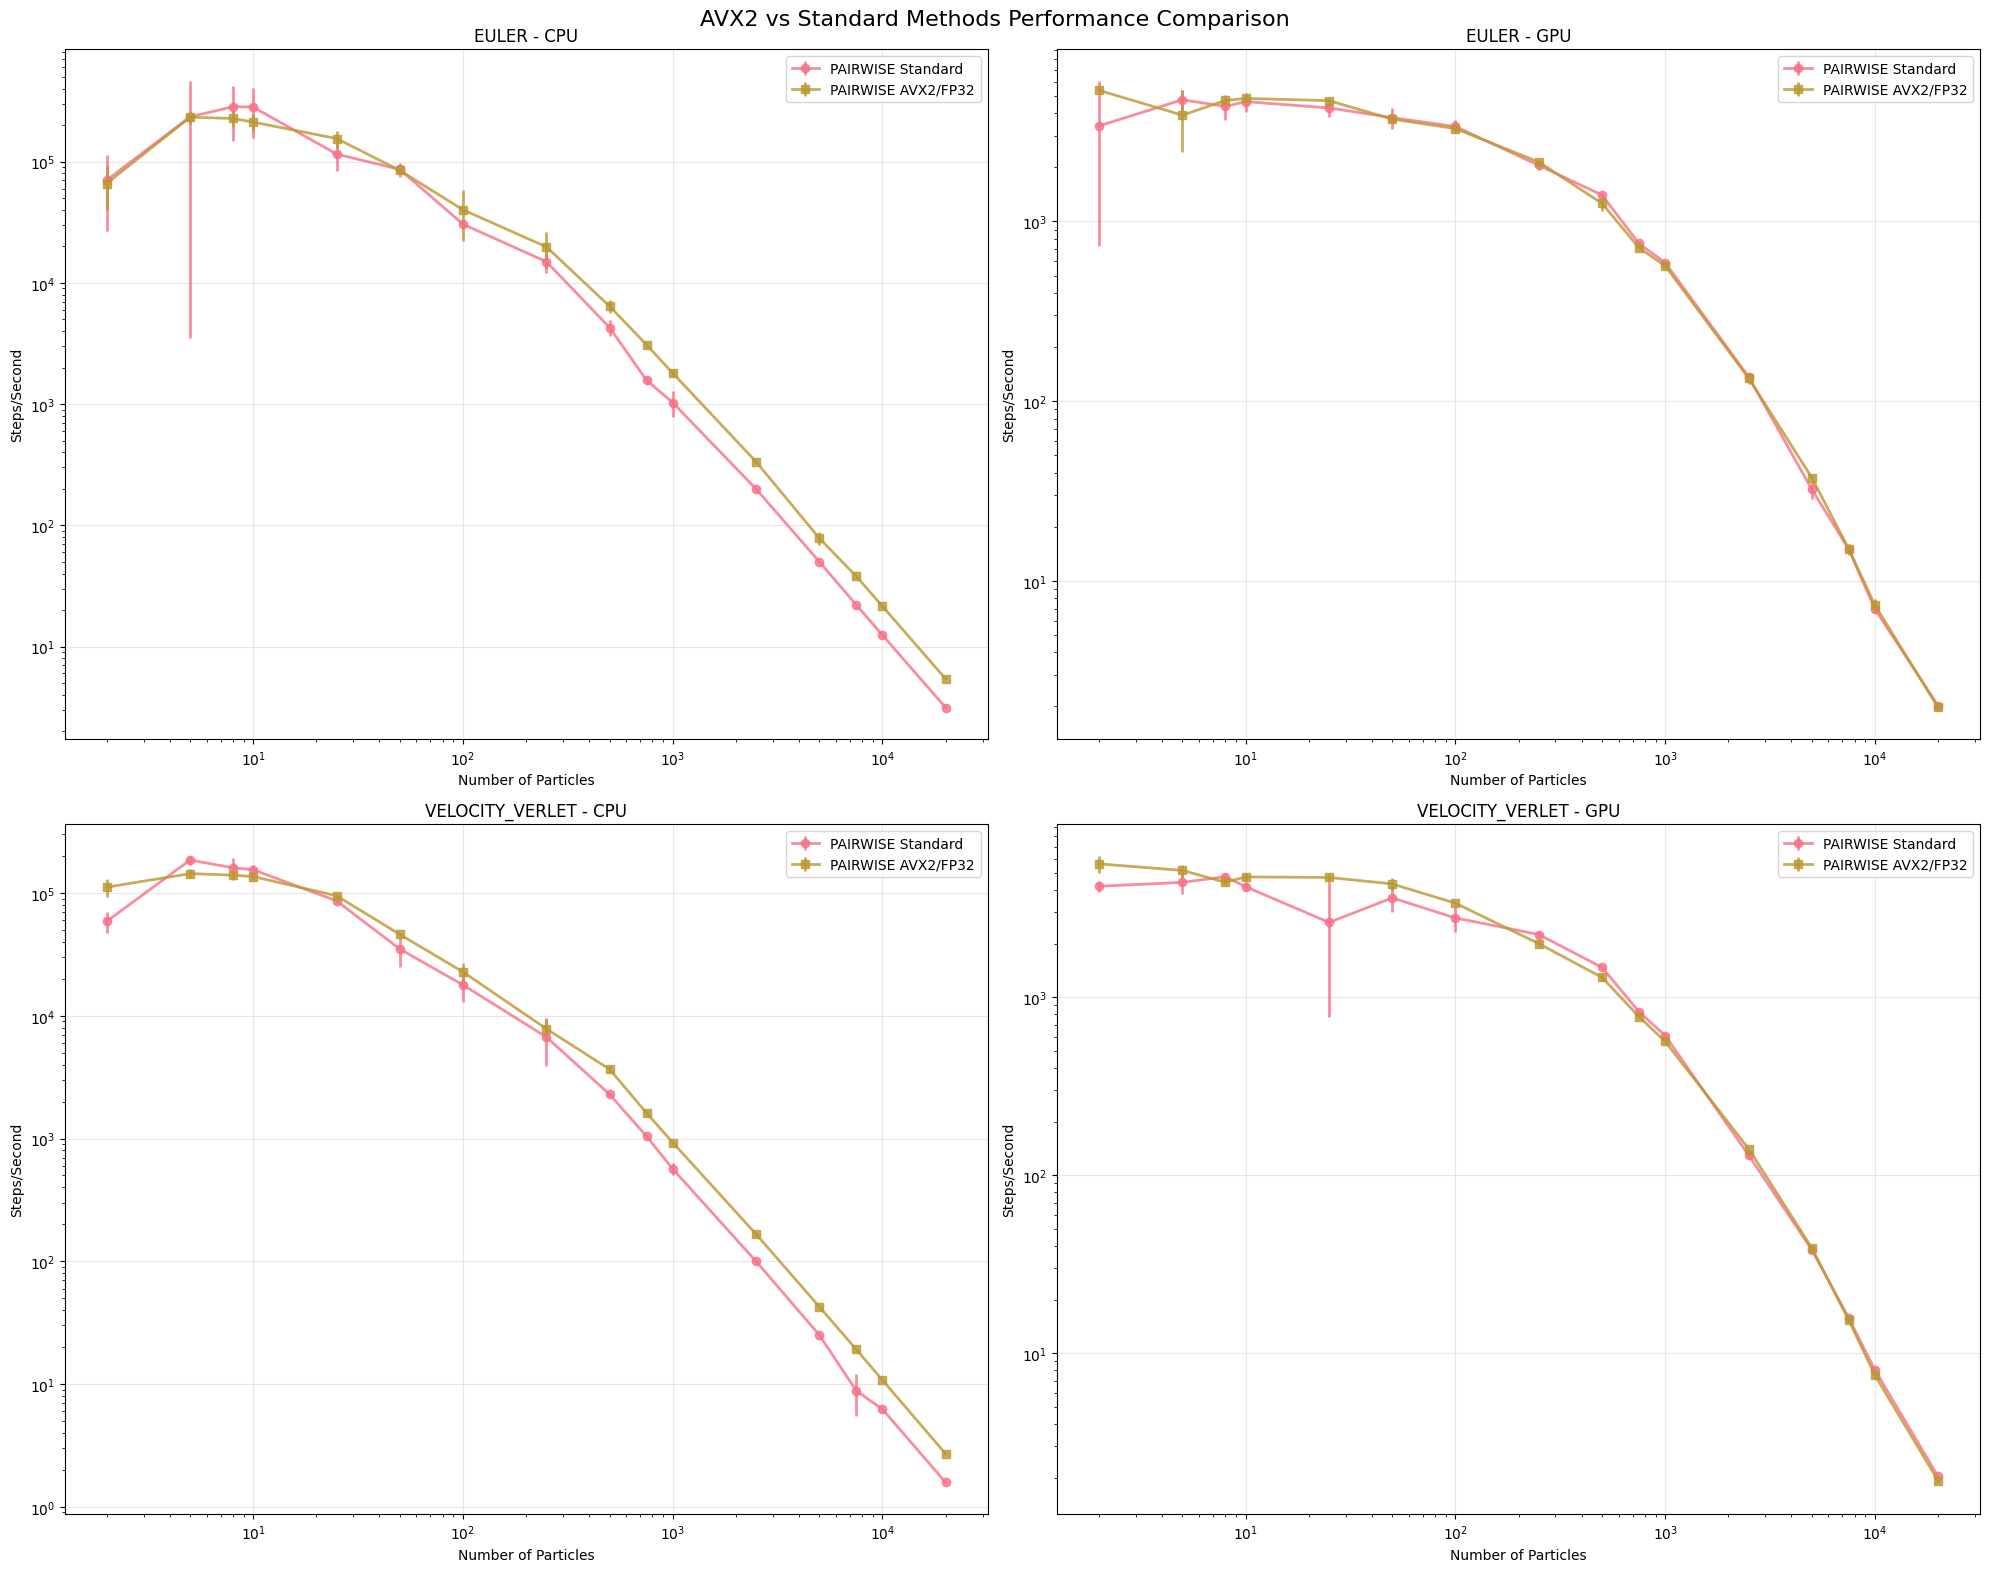
\includegraphics[width=0.85\linewidth]{figures/basic_GPU_CPU_AVX.png}
\end{frame}

\begin{frame}{Basic CPU-GPU Comparison Benchmark}
    \centering
    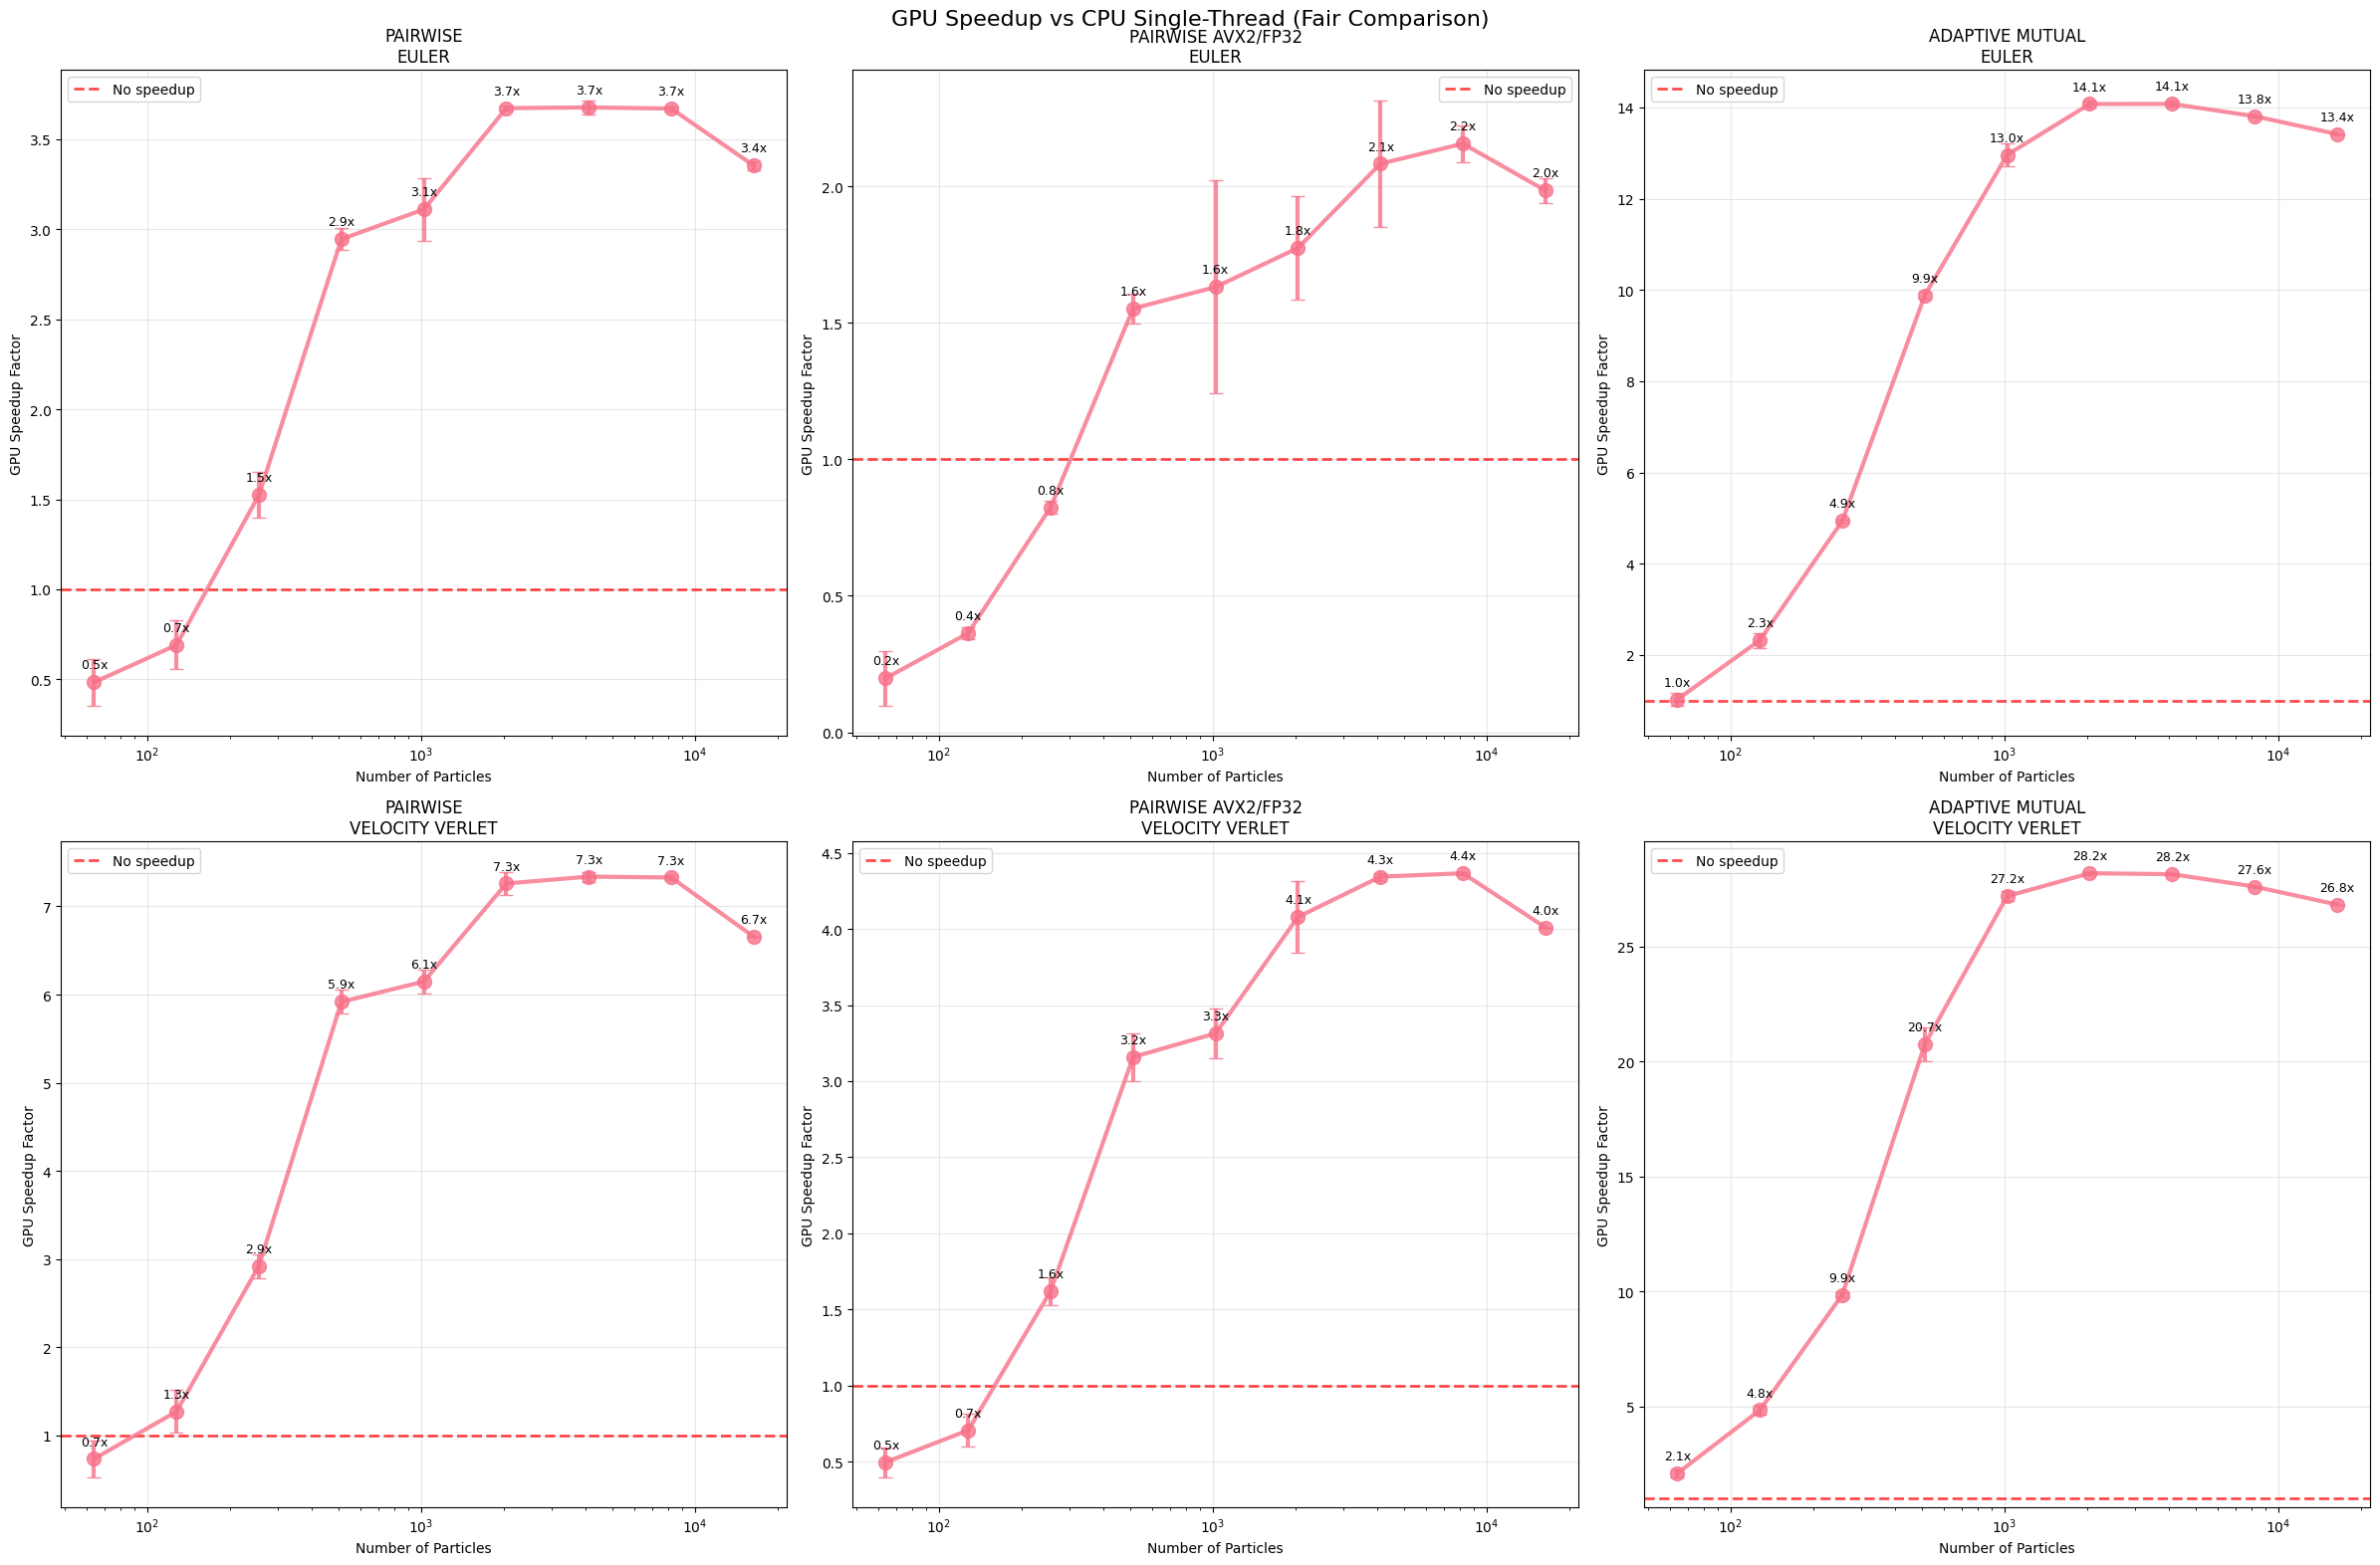
\includegraphics[width=0.99\linewidth]{figures/basic_GPU_CPU_speedup.png}
\end{frame}

\begin{frame}{CPU-Methods Comparison Benchmark}
    \centering
    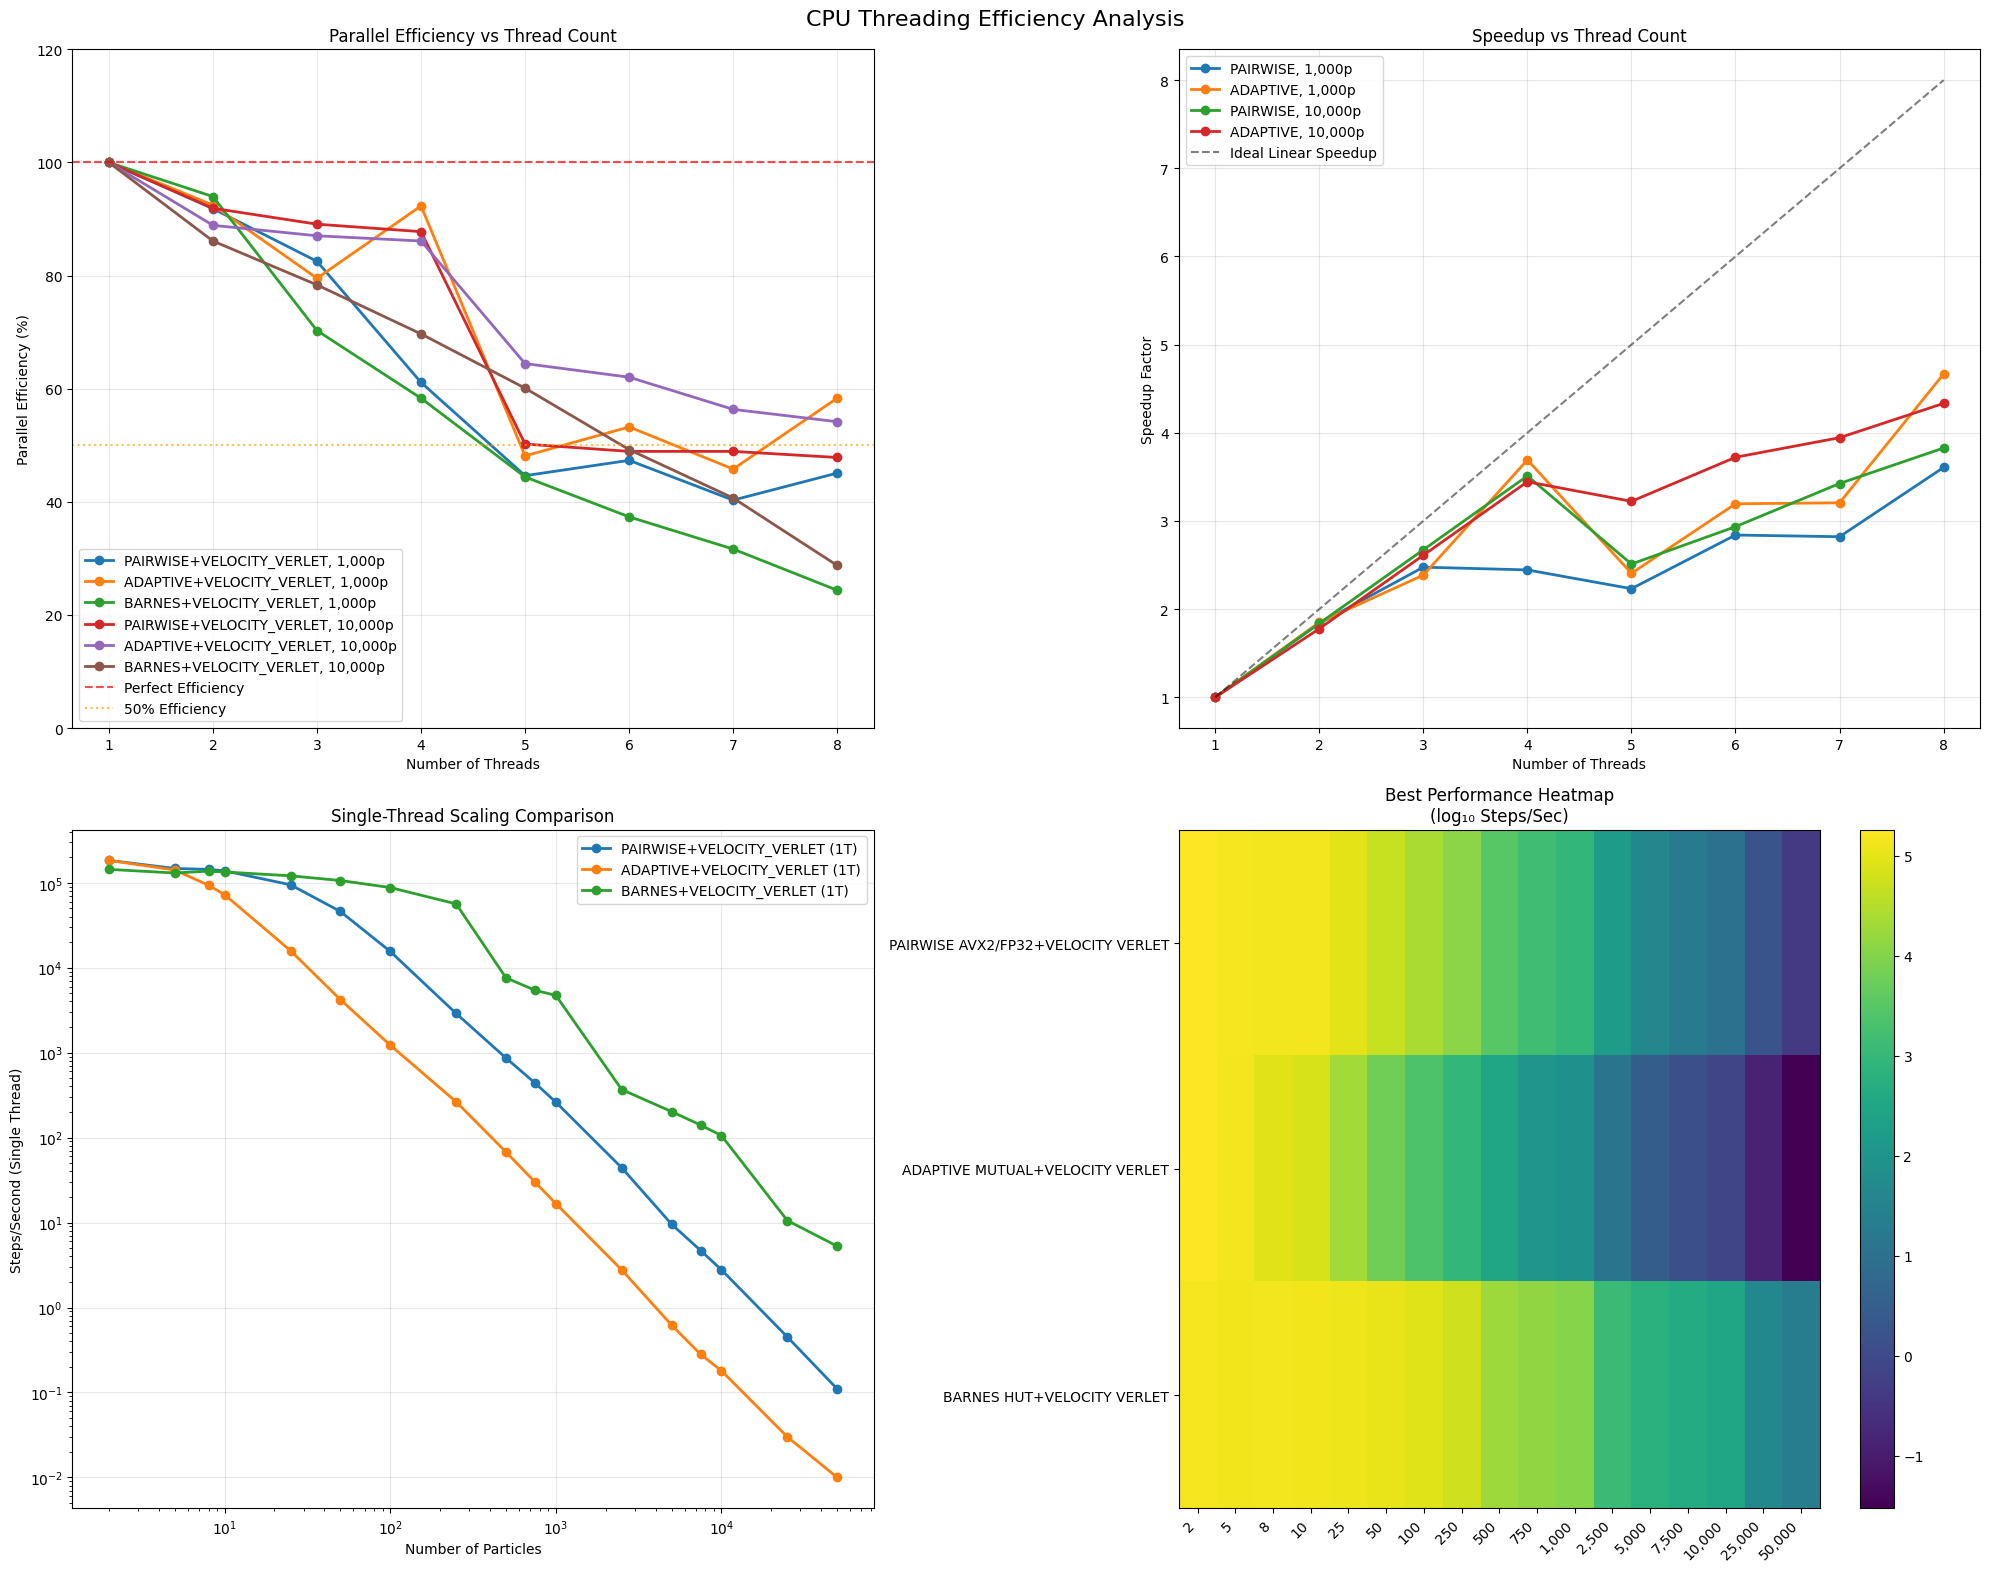
\includegraphics[width=0.85\linewidth]{figures/CPU_methods_heatmap.png}
\end{frame}

\begin{frame}{CPU-Methods Comparison Benchmark}
    \centering
    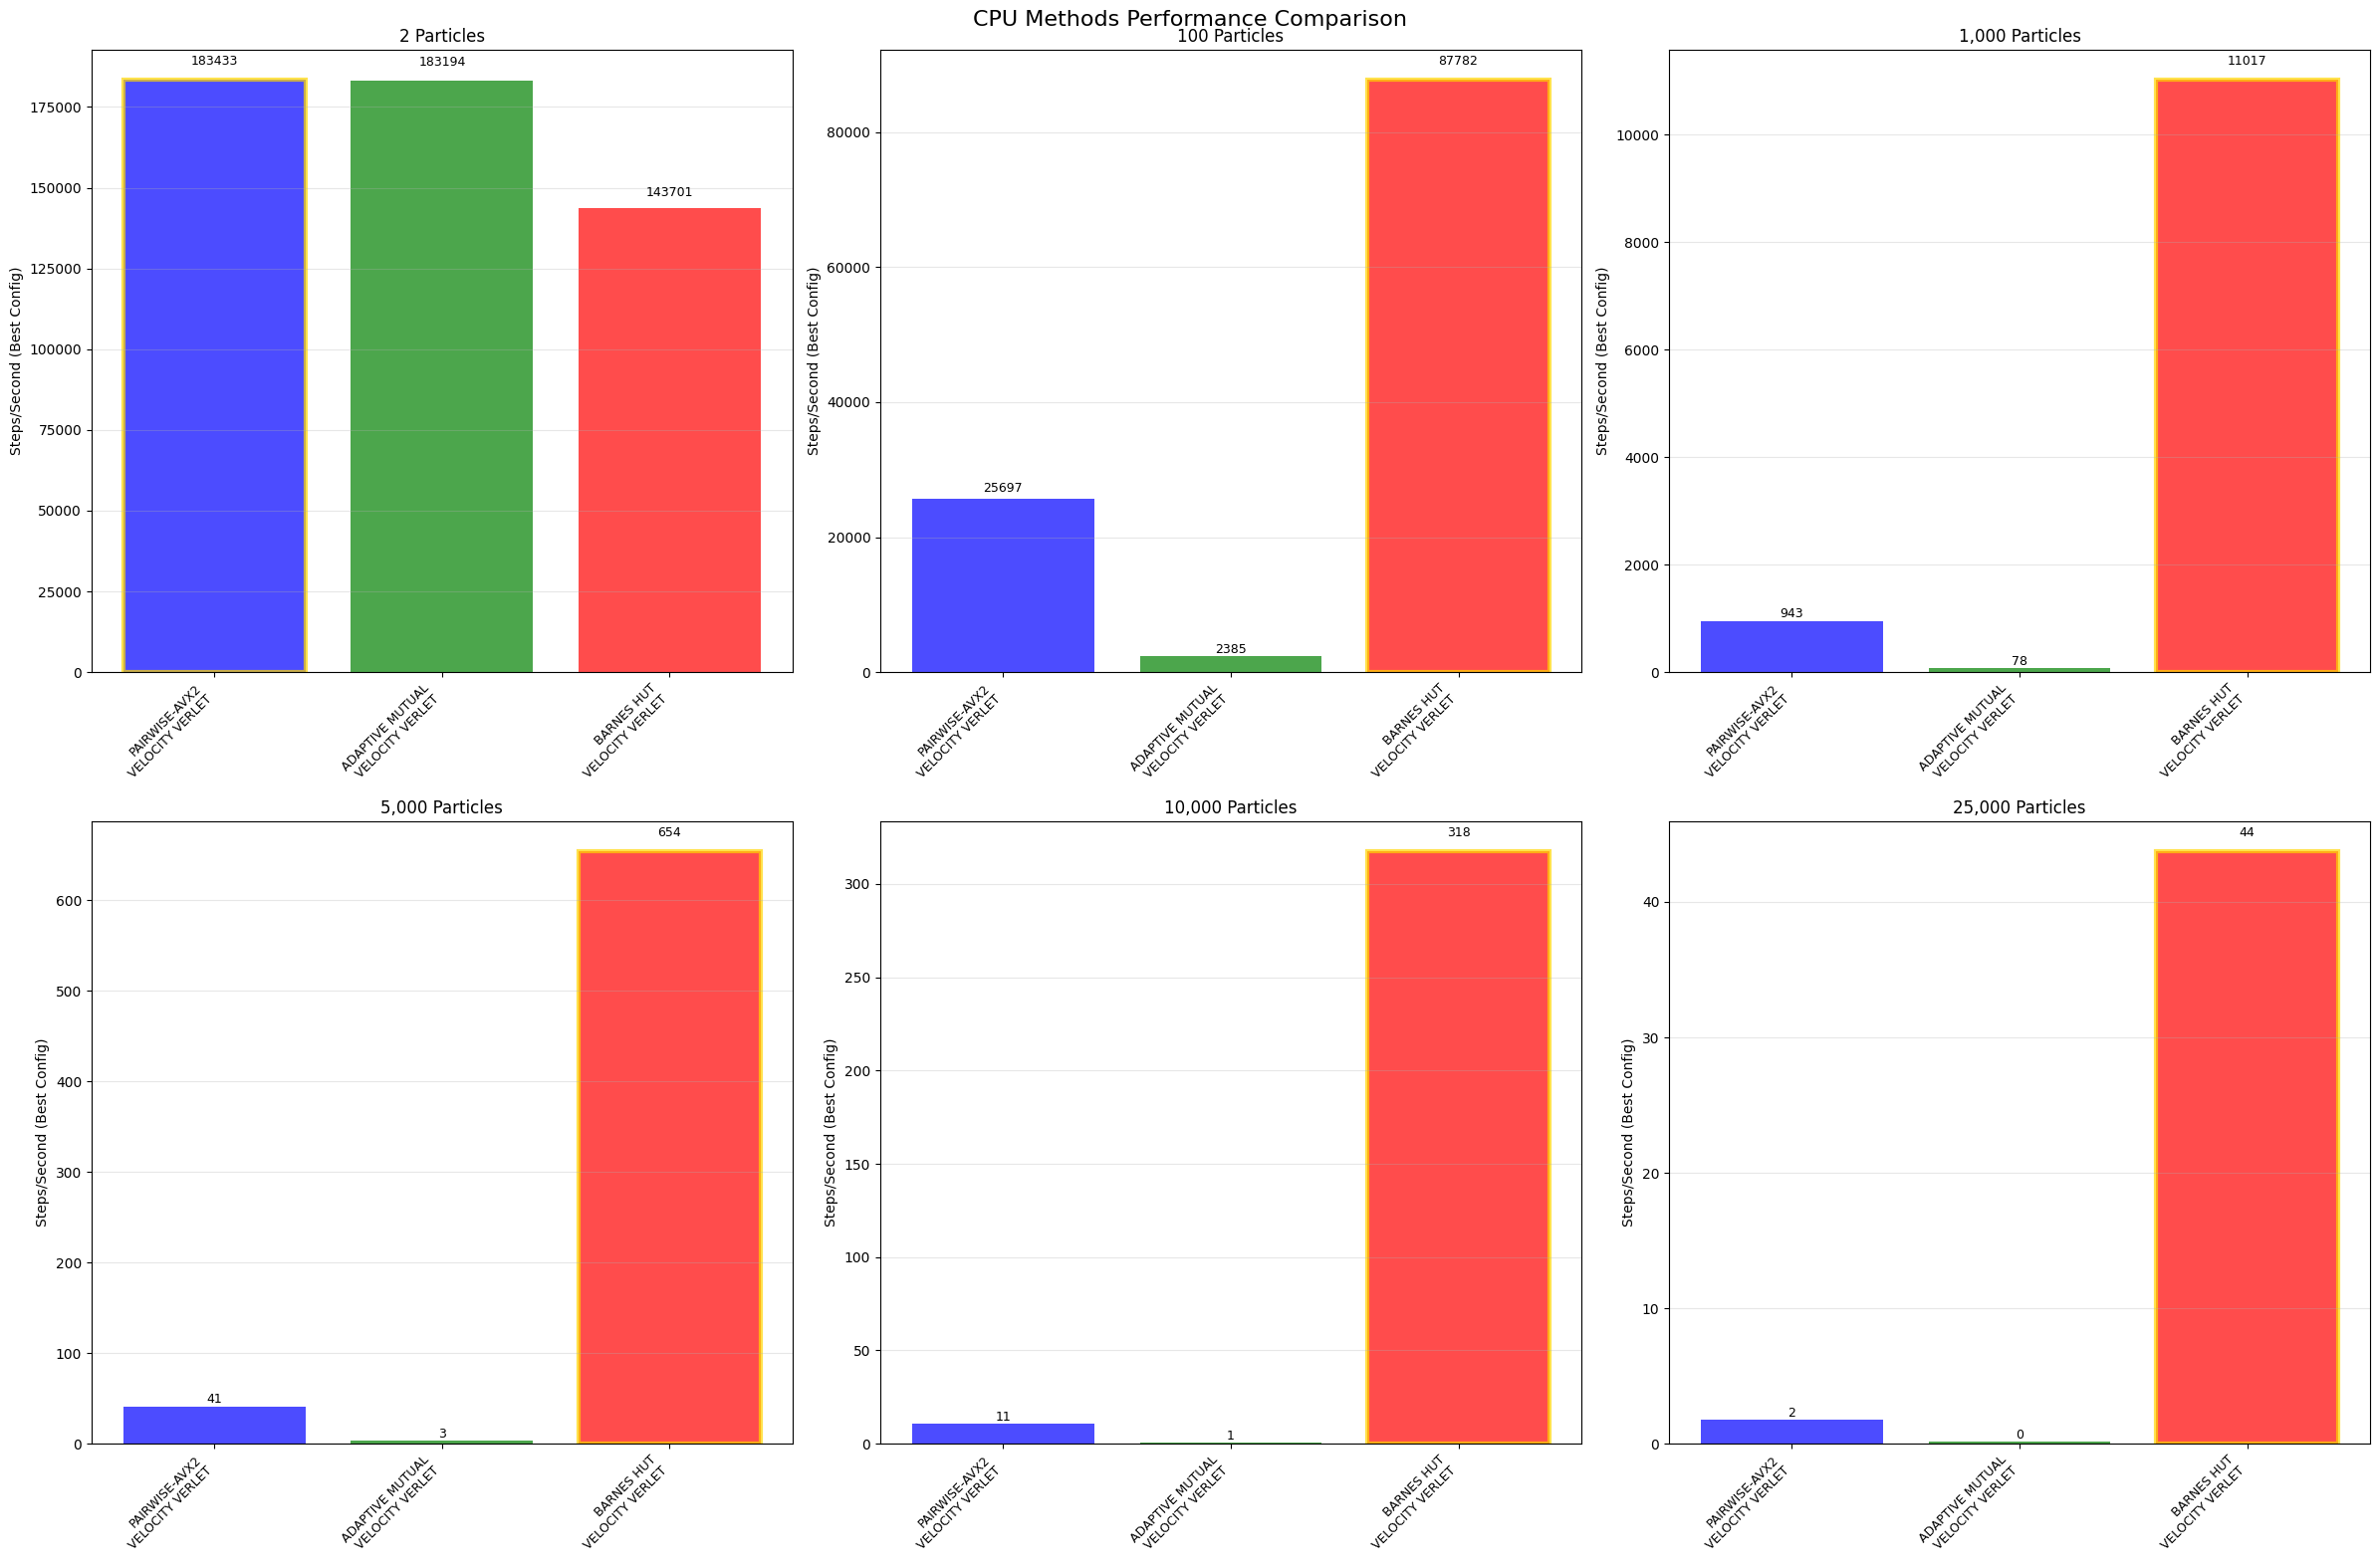
\includegraphics[width=0.99\linewidth]{figures/CPU_methods_hist.png}
\end{frame}

\begin{frame}{BH vs GPU Comparison Benchmark}
    \centering
    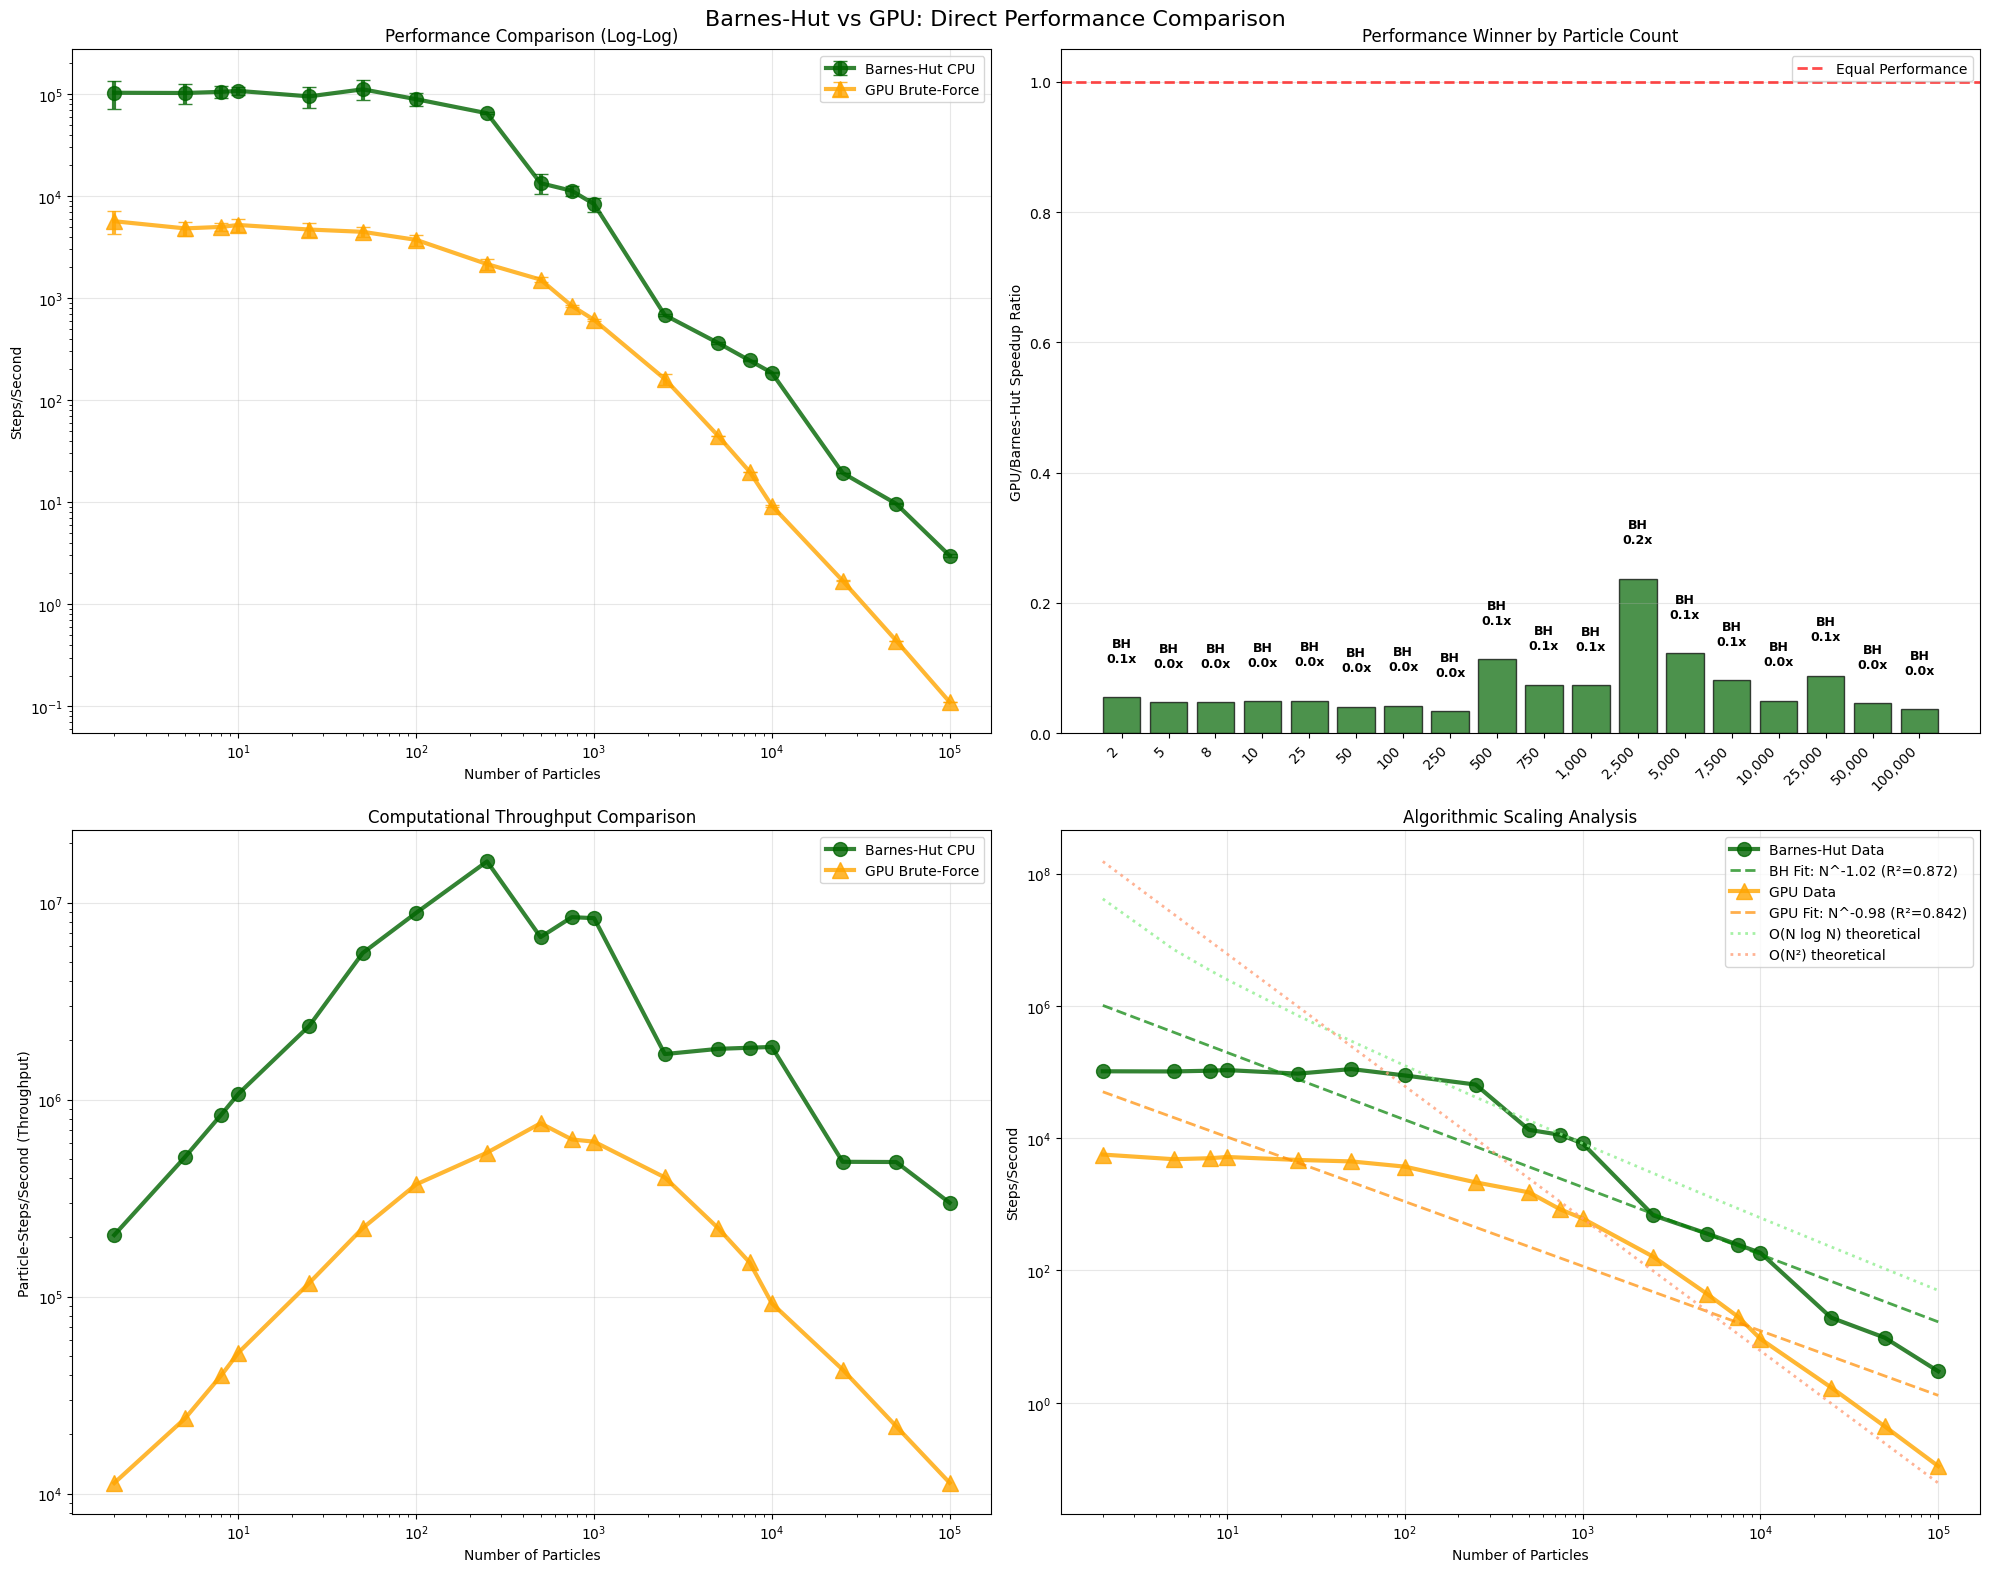
\includegraphics[width=0.85\linewidth]{figures/BH_GPU_perf.png}
\end{frame}


%\section{Visualization Stack}
%\begin{frame}{Visualization Stack}
%    \begin{itemize}
%        \item Real-time interactive visualization (OpenGL + CUDA)
%        \item Particle rendering and camera control
%        \item Output: images, videos, CSV for analysis
%    \end{itemize}
%\end{frame}

%\section{Design Choices and Tradeoffs}
%\begin{frame}{Design Choices and Tradeoffs}
%    \begin{itemize}
%        \item Modularity vs performance
%        \item CPU vs GPU fair comparison (same memory design)
%        \item Visualization vs simulation speed
%        \item Extensibility for future research
%    \end{itemize}
%\end{frame}

\section{Limitations and Lessons Learned}
\begin{frame}{Limitations and Lessons Learned}
    \begin{itemize}
        \item Bottlenecks in compute for very large N
        \item Tradeoffs between accuracy and speed (double in GPU, same memory pattern in CPU).
        \item Importance of a clear vision at the start of the project
        \item Need for a robust testing framework
        \item Make only one main entry point per external library (or as few as possible)
        \item Future improvements: a running program you can compile without looking at any library requirements
    \end{itemize}
\end{frame}

\section{Conclusions}
\begin{frame}{Conclusions}
    \begin{itemize}
        \item We skipped many small details (tiling, async memory...) in this presentation, so if you want to know more, please check the \href{}{GitHub repository} or the
        \item High-performance, modular N-body simulation achieved
        \item GPU acceleration enables large-scale experiments
        \item Framework ready for extension and research
    \end{itemize}
\end{frame}

\begin{emptyframe}
    \centering
    Thank you for your attention! \\
    Questions? \\
    Demo?
\end{emptyframe}

\end{document}